% NÃO altere as predefinições desse template!

\documentclass{ceel}

% ===========================
%Coloque aqui pacotes adicionais, se necessário
\usepackage{verbatim}
\usepackage{subfig}
%\usepackage{caption}
%\usepackage{subcaption}
\usepackage{hyperref}%
\usepackage{array}
\usepackage{booktabs}
\usepackage{float}
%\usepackage{wrapfig}
%%===========================

% Dados do trabalho
\title{Métodos de limiarização de imagens QR Code em distintos padrões de luminosidade}

% Autores: o primeiro será, necessariamente, o apresentador do trabalho
% Caso o trabalho não tenha 8 autores, exclua os campos que não foram preenchidos
\author[1]{\underline{Lesly Viviane Montúfar Berrios}\thanks{leslymontufar@ufu.br}}
\author[2]{Luciano Xavier Medeiros\thanks{lucianox@ufu.br}}
\author[2]{Alexandre Coutinho Mateus\thanks{acmateus@ufu.br}}


% Adicione as instituições de cada autor e indique corretamente no campo acima
\affil[1]{FEELT - Universidade Federal de Uberlândia}
\affil[2]{FEELT - Professor Adjunto - Universidade Federal de Uberlândia}

\begin{document}

\inserirtitulo

\begin{multicols}{2}

% Adicione o Resumo do seu trabalho no campo abaixo, com início em "O objetivo [...]"
\textbf{\emph{Resumo} - Este artigo propõe três métodos de binarização para imagens de QR Codes e, subsequentemente, realiza-se a análise de eficiência de cada técnica desenvolvida para diferentes padrões de luminosidade. Sabe-se que, intrínseco ao processo de reconhecimento de um símbolo QR, é necessária a aplicação de uma técnica de binarização, cuja eficácia depende da iluminação ambiente na qual a imagem foi exposta. Sob essa perspectiva, é de interesse avaliar quais seriam os métodos eficazes considerando-se as peculiaridades do ambiente de captura da imagem.}
\vspace*{10pt}

%Adicione as palabras-chave do seu trabalho abaixo
\textbf{\emph{Palavras-Chave} - Análise de eficiência, binarização, imagem, luminosidade, QR Code.}


\begin{center}
%Insira aqui o Título do trabalho em inglês
\noindent\textbf{\large \uppercase{Thresholding methods of QR Code images in different light patterns}}
\end{center}

%Insira aqui o resumo do seu trabalho em inglês 
\textbf{\emph{Abstract} - This paper proposes three binarization methods for QR Codes images and, subsequently, the efficiency analysis of each technique developed for different light patterns is performed. It is known that, intrinsic to the process of recognizing a QR symbol, it is necessary to apply a binarization technique, whose effectiveness depends on the ambient lighting in which the image was exposed. Therefore, it is of interest to evaluate which methods would be best considering the peculiarities of the shooting environment.} 
\vspace*{10pt}

%Insira aqui as palavras-chave do seu trabalho em inglês
\textbf{\emph{Keywords} - Efficiency analysis, image, light, QR Code, thresholding.}

%Introdução: Caso queira pode mudar o título da seção para qualquer outro. Dentro das chaves insira o título da seção e abaixo insira o texto da mesma.
\section{Introdução}
Com surgimento no Japão em 1994, os \textit{Quick Response Codes} (\textit{QR Codes}) são marca registrada da empresa Denso-Wave Incorporated, uma subsidiária da Toyota, cujo propósito de criação estava em facilitar o processo de catalogação de componentes automobilísticos \cite{denso}. Entretanto, sua utilização não se ateve a essa finalidade, devido à grande velocidade em que podem ser lidos e decodificados eletronicamente. Além disso, é uma ferramenta que tem sido bastante difundida mundialmente, em virtude do rápido desenvolvimento de dispositivos portáteis capazes de ler QR Codes e ao crescente uso comercial associado, em especial, à área de marketing.

Em termos práticos, a utilização de telefones celulares, câmeras digitais ou outros equipamentos para a coleta da imagem de código QR pode apresentar empecilhos significantes para o reconhecimento do símbolo, ocasionados tanto por fatores do ambiente, quanto pela forma de manuseio do usuário. Sob essa perspectiva, o ambiente de captura mostra-se como aspecto de bastante relevância e associa-se, principalmente, às irregularidades da iluminação. Outrossim, o manuseio do equipamento pelo usuário pode provocar distorção geométrica, problemática amenizada como propõe, por exemplo, 
Wei et al. \cite{jin-wei}, por meio de um método de correção de imagem
de código QR com base em morfologia, que consiste na obteção de informações relativas à geometria de topologia de um conjunto desconhecido a partir de outro conjunto bem definido, e Transformada de Hough, método padrão
para detecção de formas que são facilmente parametrizadas (linhas, círculos, elipses etc) em imagens digitalizadas.

Suran \cite{k-suran} desenvolveu um algoritmo de correção de imagem de código QR baseado em Algoritmo de Detecção de Canto e Casco
Convexo, utilizando binarização localizada e morfologia matemática. Chen et al. \cite{w-chen} apresentou um método de correção
de imagem de código QR de acordo com a fórmula de transformação afim, a qual é frequentemente utilizada para corrigir distorções causadas pela rotação da câmara. Jin et al. \cite{j-chen} propôs algoritmo de correção de
imagem de código QR baseado na transformada wavelet, que consiste basicamente na decomposição dos dados de forma a possibilitar a análise tanto no domínio da frequência quanto no do tempo.

A temática deste artigo, no entanto, contempla os obstáculos devido a padrões de iluminação irregulares. Ademais, deve-se atentar ao tipo de imagem que se espera trabalhar, ou seja, comumente de baixo contraste, o que é relevante na escolha do processamento adequado. Por isso, idealizou-se três métodos baseados na limiariação, os quais foram aplicados e recolhidos dados sobre imagens QR Code expostas a padrões de iluminação diferentes. Dessa maneira, propõe-se verificar o nível de correspondência de imagens de código QR submetidas a métodos de binarização distintos, para assim poder determinar o mais eficiente e estabelecer uma relação com o ambiente de captura.

Na Seção \ref{caracteristicas} serão apresentadas características básicas dos QR Codes. Na Seção \ref{metodologia}, o procedimento realizado para a coleta de imagens e exemplificação do impacto provocado pela iluminação irregular Já na Seção \ref{metodos}, são descritos e exemplificados os algoritmos das técnicas de binarização desenvolvidas, assim como realizada a análise de eficiência para as imagens do exemplo. Finalmente, na Seção \ref{resultados}, discute-se acerca dos resultados obtidos com os métodos propostos neste artigo.

\section{Características dos Códigos QR} \label{caracteristicas}
O codificação QR baseia-se na disposição de pequenos quadrados, normalmente de cores preta e branca, os quais são chamados de \textit{módulos}. Tem-se também que o tamanho do código é determinado pelo número da versão, considerando que a Versão 1 possui dimensão de $21\times21$ módulos e para as versões subsequentes há o acréscimo linear de 4 módulos, ou seja, a Versão 2 possui dimensões de $25\times25$ módulos, a Versão 3, $29\times29$ módulos, e assim por diante. 

QR Codes contêm também uma técnica de correção de erro que, a partir da inserção de dados redundantes à imagem, permite a extração da informação contida no código, mesmo que a superfície no qual foi impresso esteja danificada. Logo, quanto maior a capacidade de correção, menor o espaço para o armazenamento de dados. A Tabela \ref{nivel-correcao} descreve os 4 possíveis níveis de correção de erro.

\vspace{0.15cm}
\begin{minipage}[h]{\columnwidth}
\begin{scriptsize}
    \def\arraystretch{1.35}
    \captionsetup{type=table}
    \begin{center}
    \caption{Níveis de Correção de Erro.} \label{nivel-correcao}
    \vspace{-0.2cm}
    \begin{tabular}{ c  c } \toprule
    \textbf{Nível de correção de erro}&  \textbf{Capacidade de correção}\\\midrule
     L & Recupera 7\% dos dados \\
    M & Recupera 15\% dos dados \\
    Q & Recupera 25\% dos dados \\
    H & Recupera 30\% dos dados \\\bottomrule
    \end{tabular}
    \end{center}
\end{scriptsize}
\end{minipage}
\vspace{0.12cm}

Conforme a Figura \ref{regioes}, a estrutura do código constitui-se de duas principais regiões: \textit{região de codificação} e \textit{elementos funcionais}. A região de codificação inclui a \textit{Format Information} e \textit{Version Information}, além das \textit{Data Codewords} e \textit{Error Correction Codewords}. Já os elementos funcionais são compostos pelo \textit{Finder Patterns}, \textit{Separator}, \textit{Timing Patterns} e \textit{Alignment Patterns}. Assim, quando uma imagem de QR Code é capturada, busca-se por esses padrões para o reconhecimento e decodificação rápida dos dados \cite{qr-tutorial}.

\section{Metodologia} \label{metodologia}

\subsection{Coleta das imagens QR Code}

Foram gerados 13 QR Codes, de versões e níveis de correção de erro distintos (Veja Tabela \ref{qrtable}), e impressos em folhas A4, sendo 4 imagens por página, só frente, fato que influencia no tamanho da imagem a ser coletada, por conseguinte, em sua resolução. Em seguida, buscou-se locais com diferentes padrões de luminosidade, a fim de simular variadas 
situações problema enfrentadas pela tecnologia de reconhecimento.

\hspace{-0.45cm}
\begin{minipage}[h]{\columnwidth}
%\captionsetup{type=figure, singlelinecheck=off, justification=raggedright, margin=0pt, font=footnotesize}
\captionsetup{type=figure, margin=5pt}
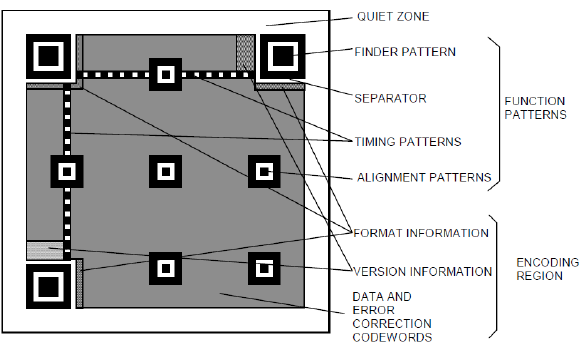
\includegraphics[width=\columnwidth]{regioes-qr-upercase}
\caption{\label{regioes}Regiões de um QR Code, ilustrado em símbolo da Versão 7 \cite{chines}.} 
\end{minipage}
\vspace{0.25cm}

Escolhidos três ambientes, utilizou-se a camêra de um celular (\emph{Samsung SM-J730G}) de $13\ Mpx$ para realizar a captura dos QR Codes impressos. Assim, obteve-se 39 imagens no formato \emph{jpg} de resolução  $4128 \times 3096$. 
Na Figura \ref{exemplo} há um exemplo de coleta de imagens de um QR Code em específico, que corresponde ao QR Code 3 descrito na Tabela \ref{qrtable}, que foi submetido aos três padrões de luminosidade utilizados nesse artigo para teste dos métodos de binarização propostos.

É evidente nas Figuras \ref{exemplo}(a) e (b) que QR Codes expostos a iluminações mais uniformes tendem a apresentar histogramas com dois picos, um representando os módulos mais escuros e o outro, os mais claros. Constata-se ainda, nas Figuras \ref{exemplo}(c) e (d), que imagens advindas de iluminações próximas a um degradê dispõem de histogramas com mais picos. Da imagem da Figura \ref{exemplo}(e) também resulta um histograma com dois picos, porém, em virtude da baixa intensidade do nível de cinza médio, há maior concentração de píxeis com intensidade pertencente ao início da escala de cinza, como mostra a Figura \ref{exemplo}(f).

\vspace{0.15cm}
\begin{minipage}[h]{\columnwidth}
\begin{scriptsize}
    \def\arraystretch{1.35}
    \captionsetup{type=table}
    \begin{center}
    \caption{QR Codes gerados.} \label{qrtable}
    \vspace{-0.2cm}
    \begin{tabular}{ c  c   c} \toprule
    \textbf{Nome da Imagem}&  \textbf{Versão}&  \textbf{Nível de Correção de Erro}\\\midrule
    QR Code 1  & 3 & L \\
    QR Code 2  & 4 & L \\
    QR Code 3  & 5 & L \\
    QR Code 4  & 6 & M \\
    QR Code 5  & 8 & H  \\
    QR Code 6  & 8 & Q  \\
    QR Code 7  & 10 & H  \\
    QR Code 8  & 12 & H  \\
    QR Code 9  & 13 & H  \\
    QR Code 10 & 17 & H  \\
    QR Code 11 & 29 & L  \\
    QR Code 12 & 38 & H \\
    QR Code 13 & 39 & Q \\\bottomrule
    \end{tabular}
    \end{center}
\end{scriptsize}
\end{minipage}

\subsection{Procedimento realizado sobre as capturas de imagem}
No fluxograma da Figura \ref{fluxograma} visualiza-se o procedimento realizado sobre cada imagem capturada, com o intuito de se obter os resultados da Seção \ref{resultados}. Após a captura da imagem, realiza-se a transformação para a escala de cinza, a fim de prepará-la para a etapa seguinte a qual consiste na aplicação do método de binarização, idealizado e descrito na Seção \ref{metodos}. Feito isso, a imagem binarizada é redimensionada para as dimensões da imagem original (arquivo \emph{jpg} utilizado para imprimir o QR Code), para assim poder compará-las e gerar a imagem diferença, cujo propósito é marcar, na cor vermelha, os píxeis de divergência entre a imagem original e a binarizada, que também são contabilizados de forma percentual para cada método aplicado.

\hspace{-0.365cm} 
\begin{minipage}[H]{\columnwidth} %%
\captionsetup{type=figure}
\subfloat[Iluminação 1]{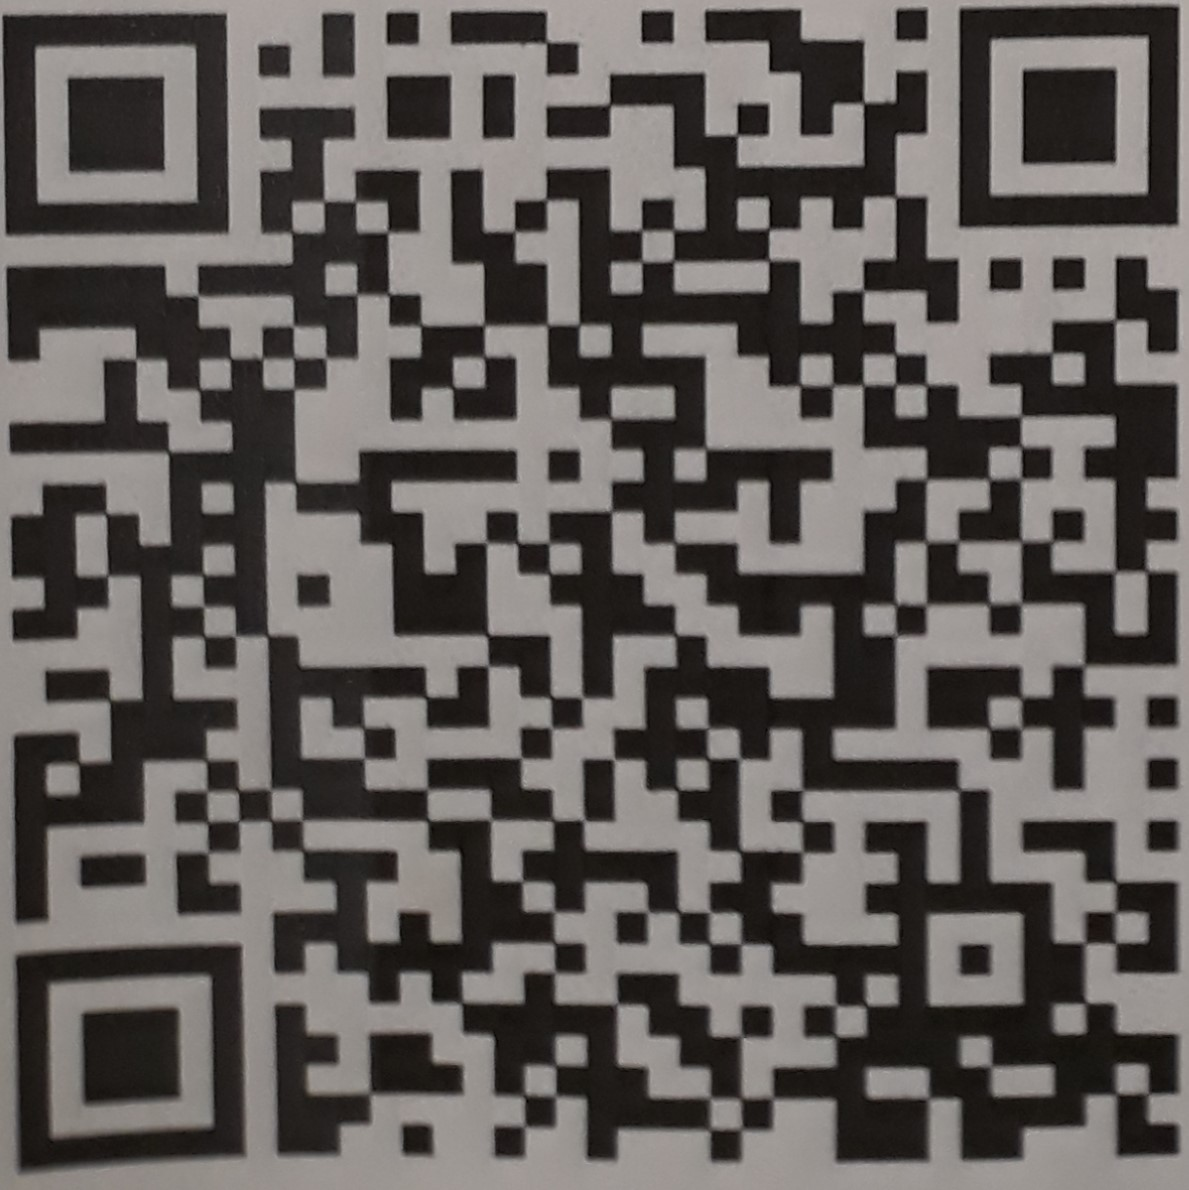
\includegraphics[width=3.5cm]{imagem03}}\hfill
\subfloat[Histograma de (a)]{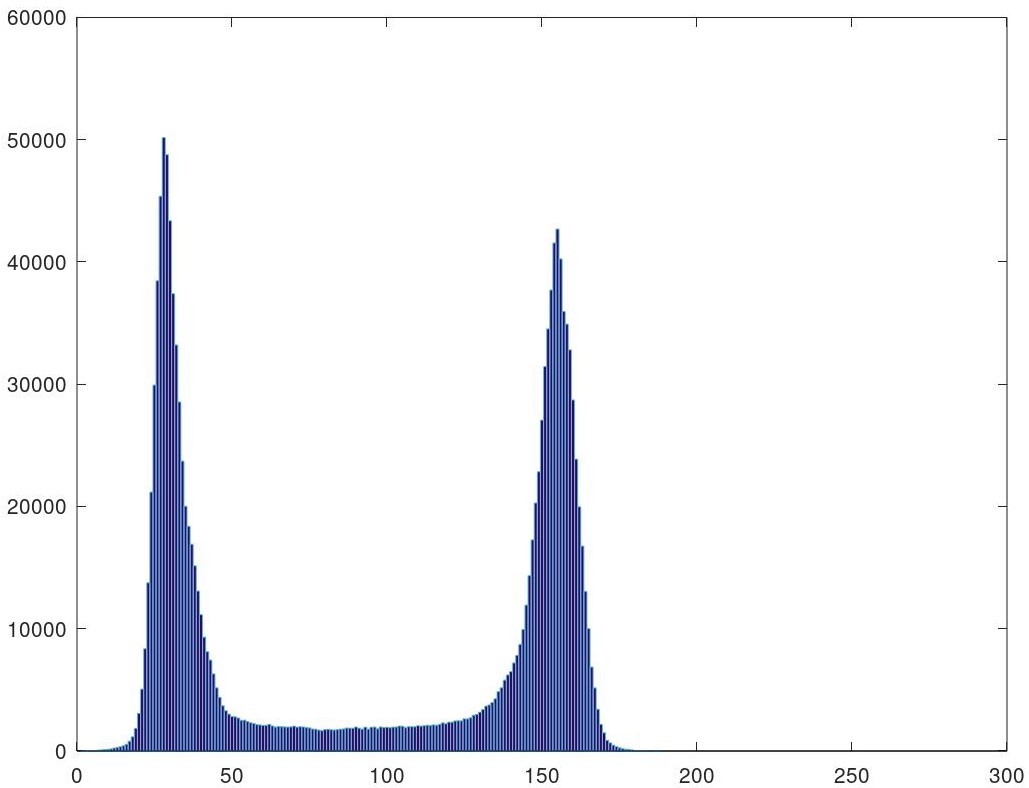
\includegraphics[width=4.52cm]{imagem03-hist}}\\
\subfloat[Iluminação 2]{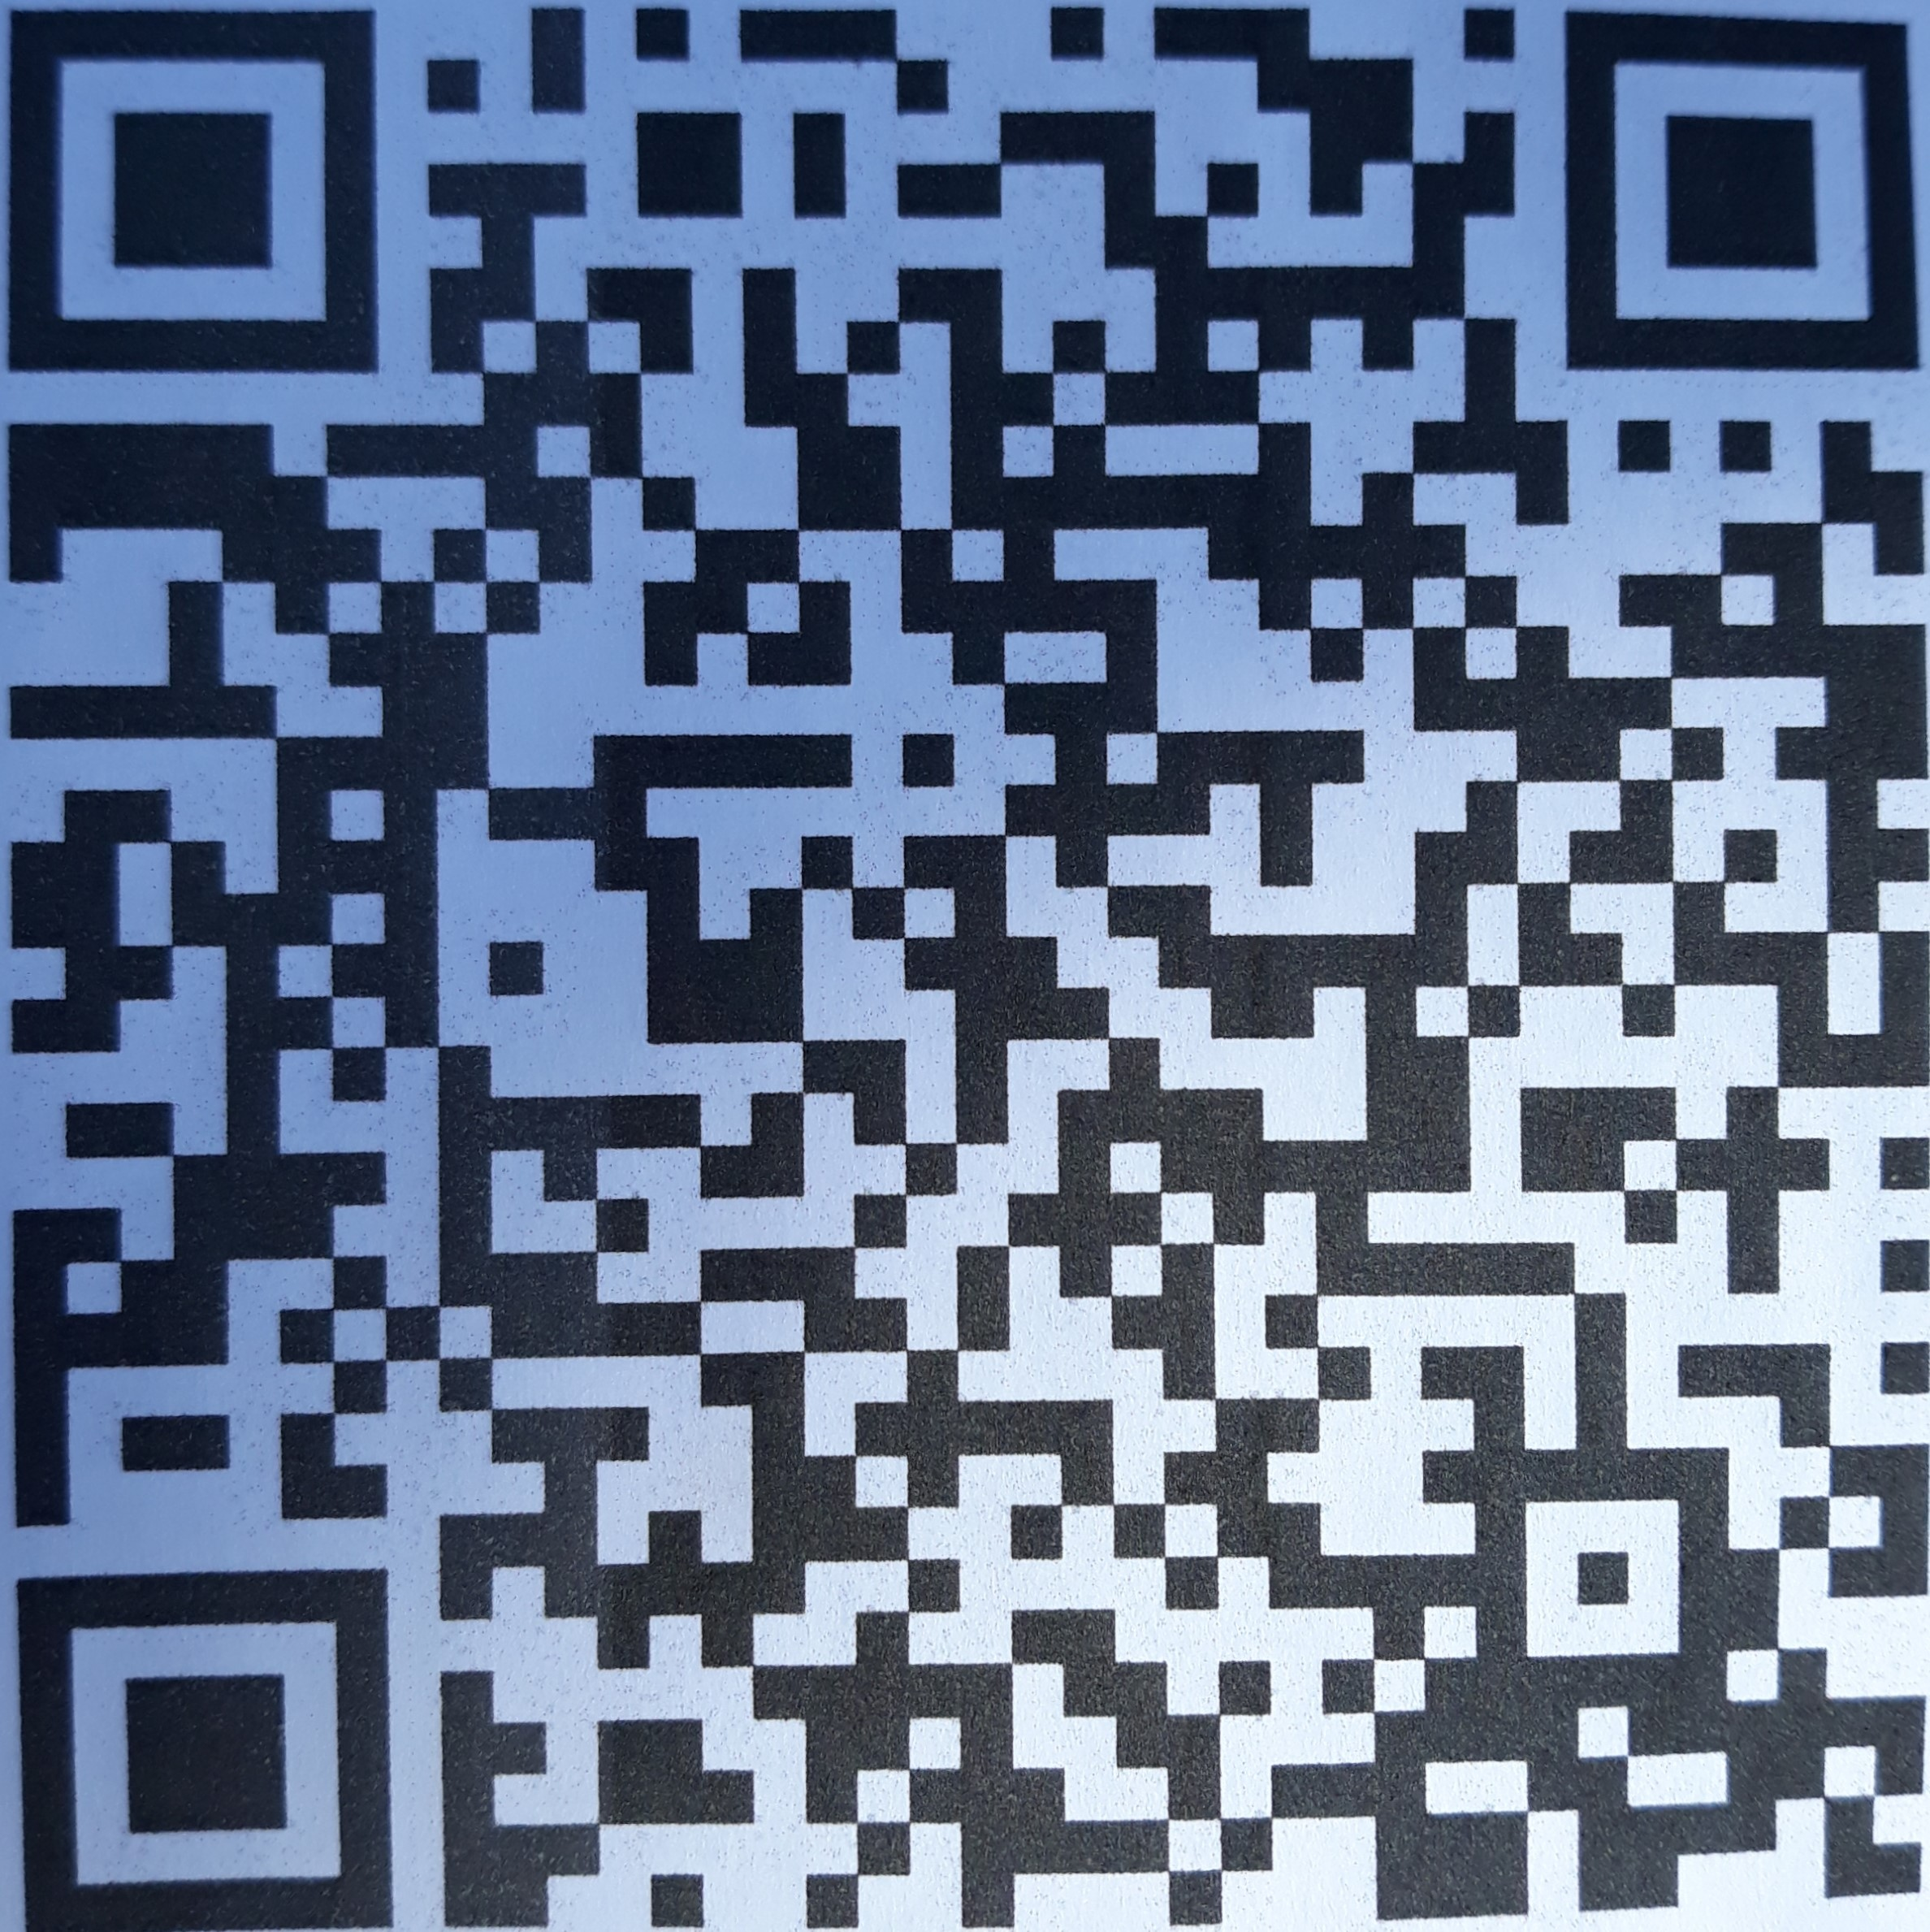
\includegraphics[width=3.5cm]{imagem16}}\hfill
\subfloat[Histograma de (c)]{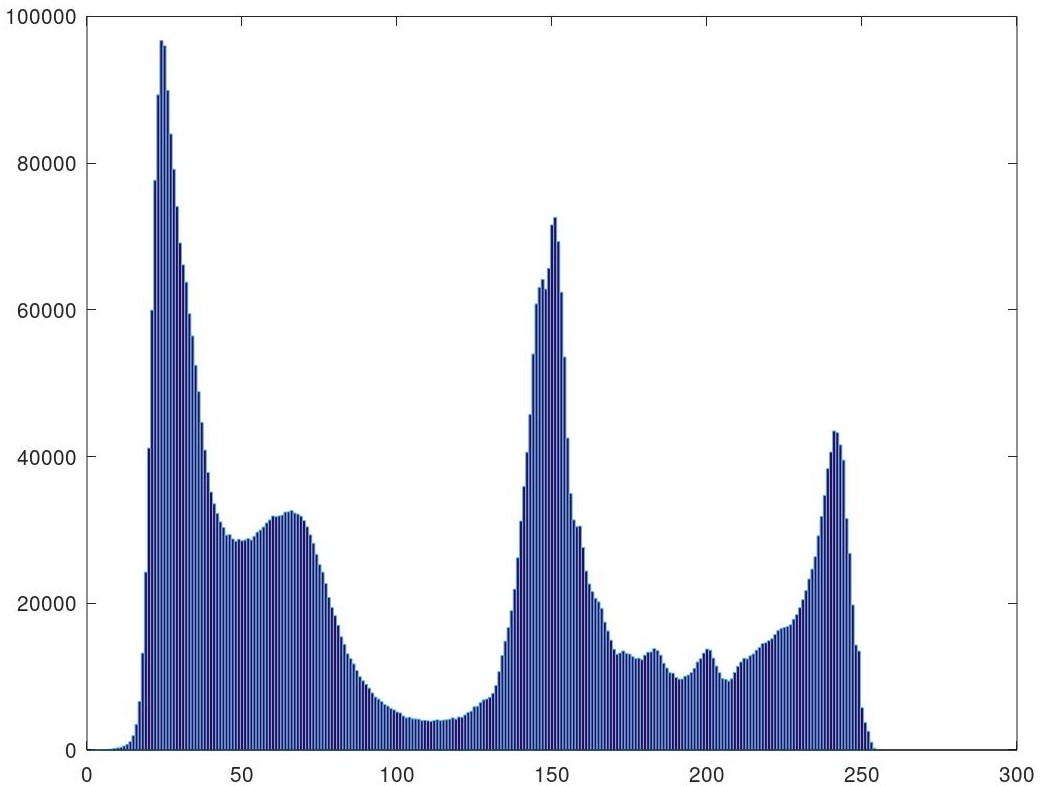
\includegraphics[width=4.52cm]{imagem16-hist}}\\
\subfloat[Iluminação 3]{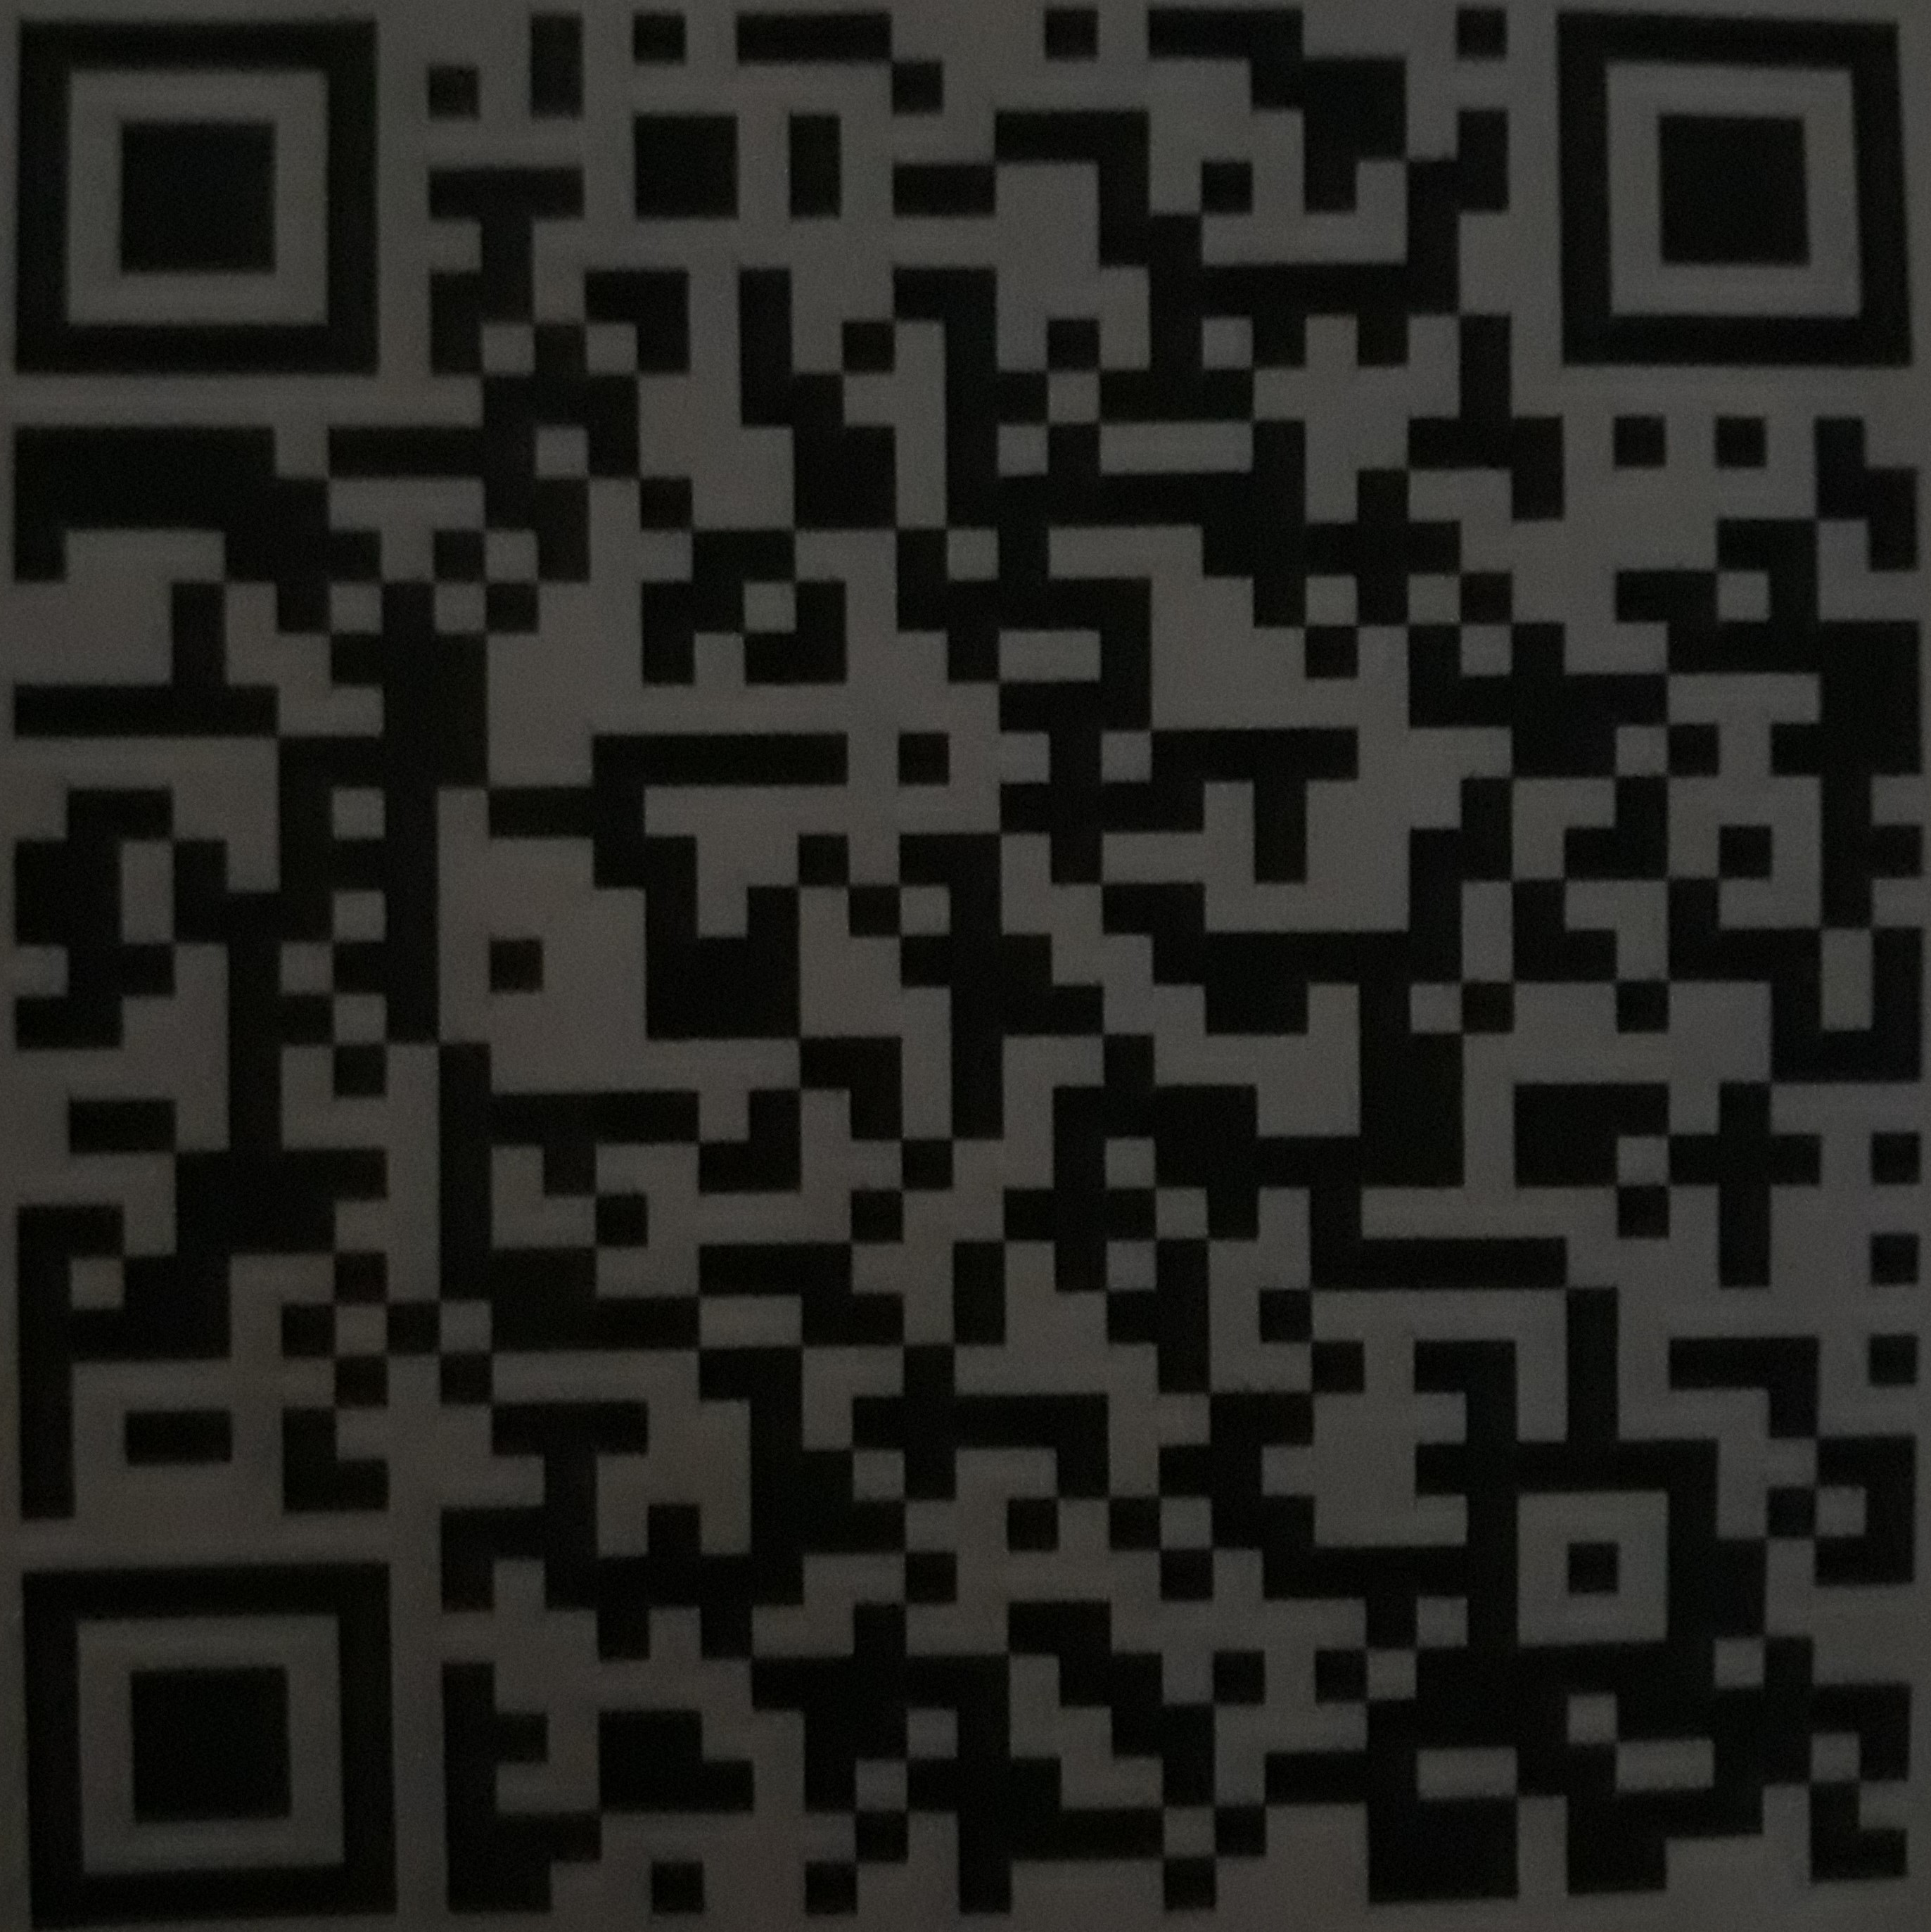
\includegraphics[width=3.5cm]{imagem29}}\hfill
\subfloat[Histograma de (e)]{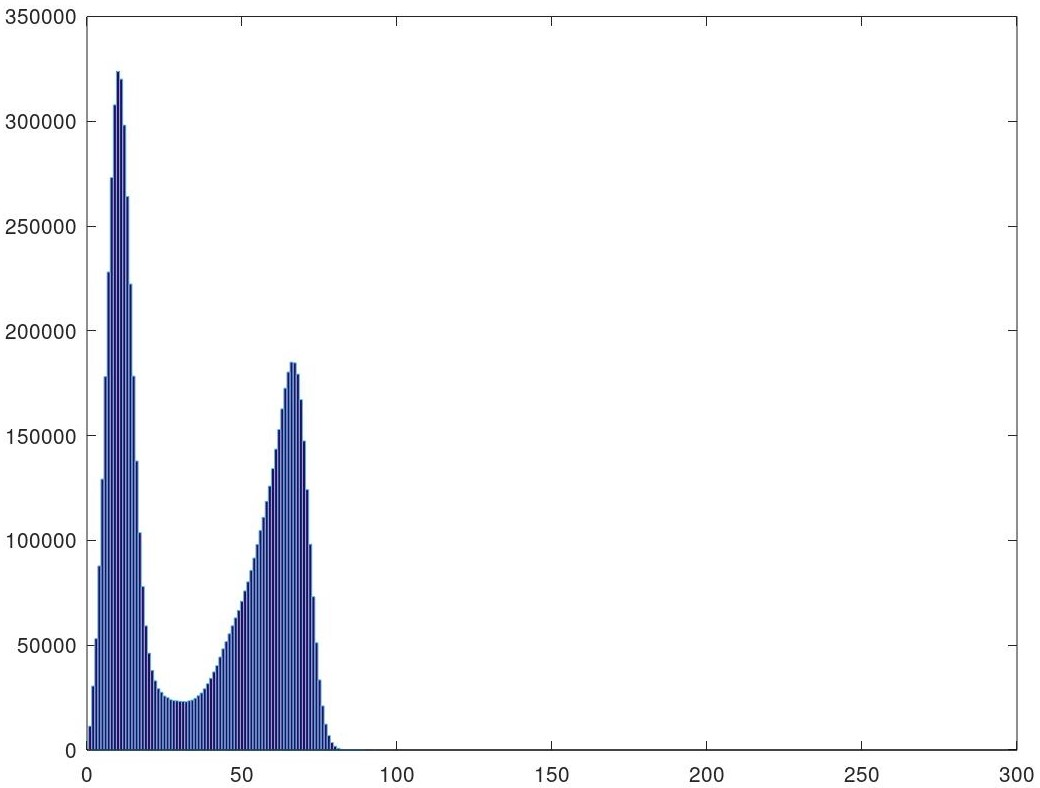
\includegraphics[width=4.52cm]{imagem29-hist}}
\vspace{-0.05cm}
\caption{Exemplos de imagens de um mesmo QR Code nos três diferentes padrões de iluminação e seus respectivos histogramas.}
\label{exemplo}
\end{minipage}

\vspace{0.5cm}
\begin{minipage}[h]{\columnwidth}
\centering
\captionsetup{type=figure}
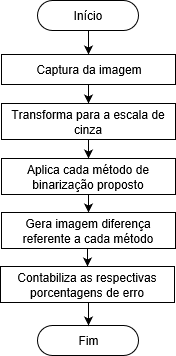
\includegraphics[scale=0.58]{Fluxograma}
\caption{Fluxograma do procedimento realizado sobre cada imagem.} \label{fluxograma}
\end{minipage}
\columnbreak

\section{Métodos de Binarização de QR Code} \label{metodos}
A \emph{binarização} (ou \emph{limiarização}) é uma função de transformação de intensidade baseadas em pontos de corte ou limiares. Dada uma imagem em nível de cinza $f(x, y)$, a binarização, no caso da utilização de somente um limiar $T$ (do inglês \emph{Threshold}), resultará em uma imagem $g(x, y)$  de dois níveis ou binária, descrita matematicamente pela Equação (\ref{Threshold}).

\begin{gather}
g( x,\ y) =\begin{cases}
0 & \quad \quad \text{se }\ f( x,\ y) \leqslant T\\
255 & \quad \quad \text{se }\ f( x,\ y)  >T
\end{cases}
\label{Threshold}
\end{gather}
%\vspace{0.1cm}

\noindent onde 0 e 255 são, respectivamente, as cores preta e branca para imagens em níveis de cinza codificadas em 8 bits.\\

São propostos, neste trabalho, os seguintes métodos: \emph{Binarização por Limiar}; \emph{Binarização Pós Equalização por Histograma}; \emph{Binarização em Sub-Regiões}. A seguir, são descritos os métodos desenvolvidos e utiliza-se imagens de um mesmo QR Code para melhor compreensão, as quais apresentam interessantes condições de iluminação (Veja Figura \ref{exemplo}).


\subsection{Binarização por Limiar} \label{Aconst}
A primeira técnica proposta neste artigo consiste na binarização da imagem a partir de dois limiares distintos. No \textit{Método do Limiar Fixo - LF} (\emph{LF}) tem-se 
$T=128$, valor correspondente à metade da escala de níveis de cinza de uma imagem codificada em 8 bits. Enquanto que para o \textit{Método do Limiar Variável} (LV), $T=M$,  sendo $M$ a intensidade média de nível de cinza da imagem analisada. Portanto, as funções de transformação dos métodos \textit{LF} e \textit{LV} são descritas, respectivamente, pelas Equações (\ref{eqLF}) e (\ref{eqLV}) e as Figuras \ref{figLF} e \ref{figLV} ilustram os resultados desses métodos aplicados a um mesmo QR Code.

\vspace{-0.01cm}
\begin{gather}
g_{LF}( x,\ y) =\begin{cases}
0 & \quad \quad \text{se }\ f( x,\ y) \leqslant 128\\
255 & \quad \quad \text{se }\ f( x,\ y)  >128
\end{cases}
\label{eqLF}
\end{gather}

%\vspace{0.02cm}
\begin{gather}
g_{LV}( x,\ y) =\begin{cases}
0 & \quad \quad \text{se }\ f( x,\ y) \leqslant M\\
255 & \quad \quad \text{se }\ f( x,\ y)  >M
\end{cases}
\label{eqLV}
\end{gather}
\vspace{0.01cm}

Observe, na Figura \ref{figLF}(e), que a técnica \emph{LF} sobre a imagem no padrão de Iluminação 3 obteve resultado desvantajoso, uma vez que a baixa iluminação do local levou ao escurecimento total da imagem, o que invialibiliza o reconhecimento do símbolo. Infere-se, assim, que a intensidade de todos os pixeis da imagem são inferiores a 128. Já na Figura \ref{figLV}(e), a técnica \emph{LV} revelou menor erro para esse padrão e, agora, é visível o símbolo QR (Veja Tabela \ref{tabela-erros}). 

\subsection{Binarização Pós Equalização por Histograma (EH)} \label{Bhist}
Outra técnica de binarização proposta por este artigo consiste em duas etapas. Realiza-se, primeiramente, a equalização por histograma da imagem do código QR, por meio do algoritmo descrito em Gonzalez e Woods \cite{gonzales}, para, em seguida, aplicar a binarização com limiar correspondente à intensidade
média de nível de cinza  $M$ da imagem equalizada. A Figura \ref{figEH} 
\columnbreak

\hspace{-0.43cm}
\begin{minipage}[h]{\columnwidth}
\captionsetup{type=figure}
\subfloat[]{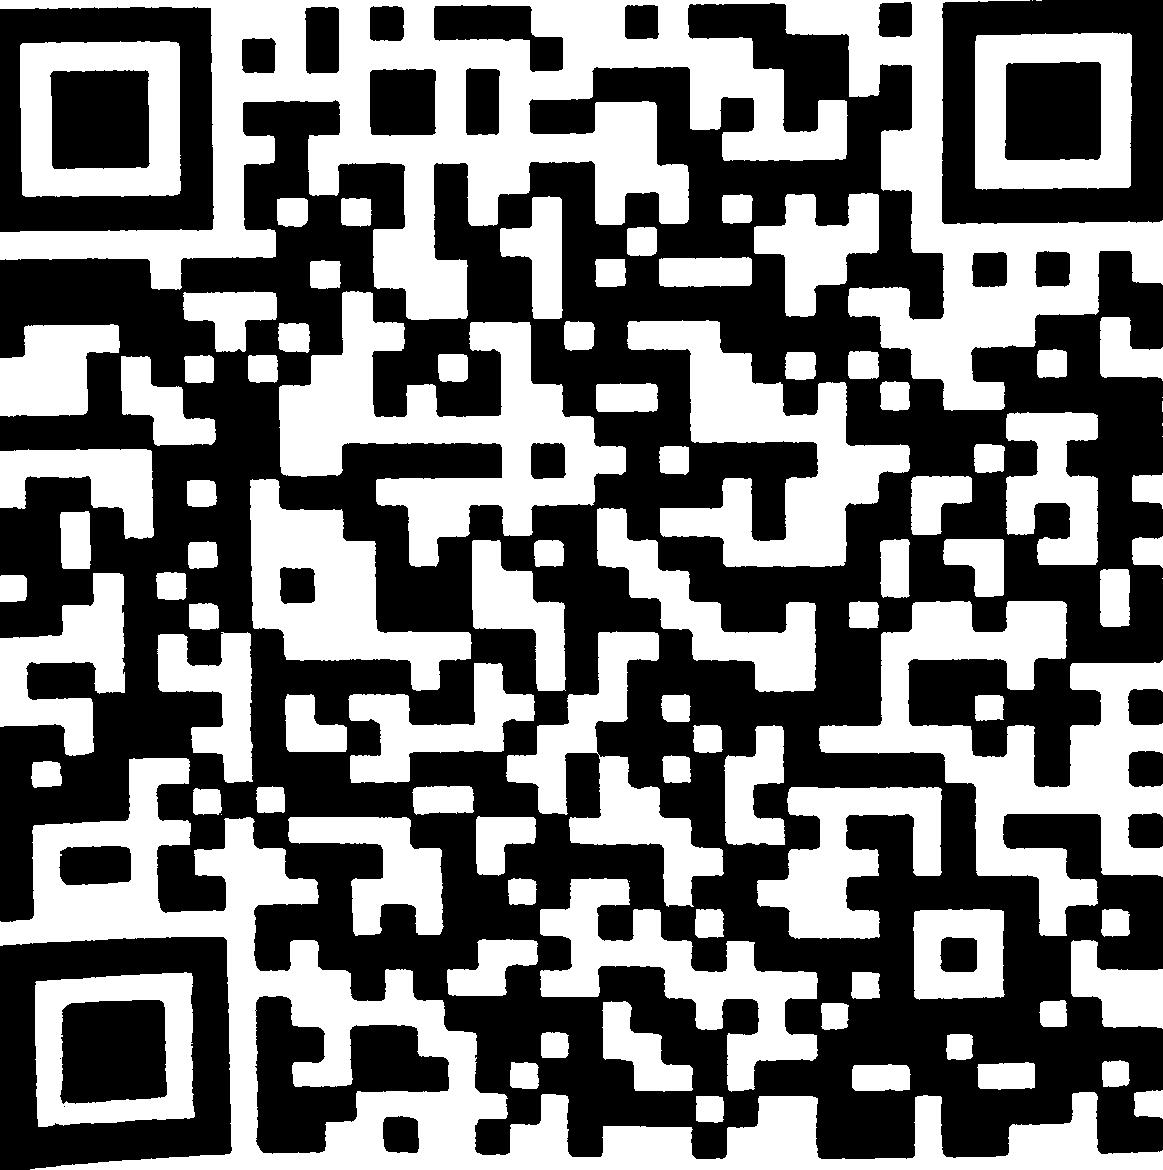
\includegraphics[width=3.68cm]{imagem03-LF}} \hfill
\subfloat[]{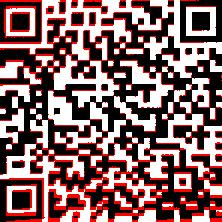
\includegraphics[width=3.68cm]{imagem03-LF-diff}}\\
\subfloat[]{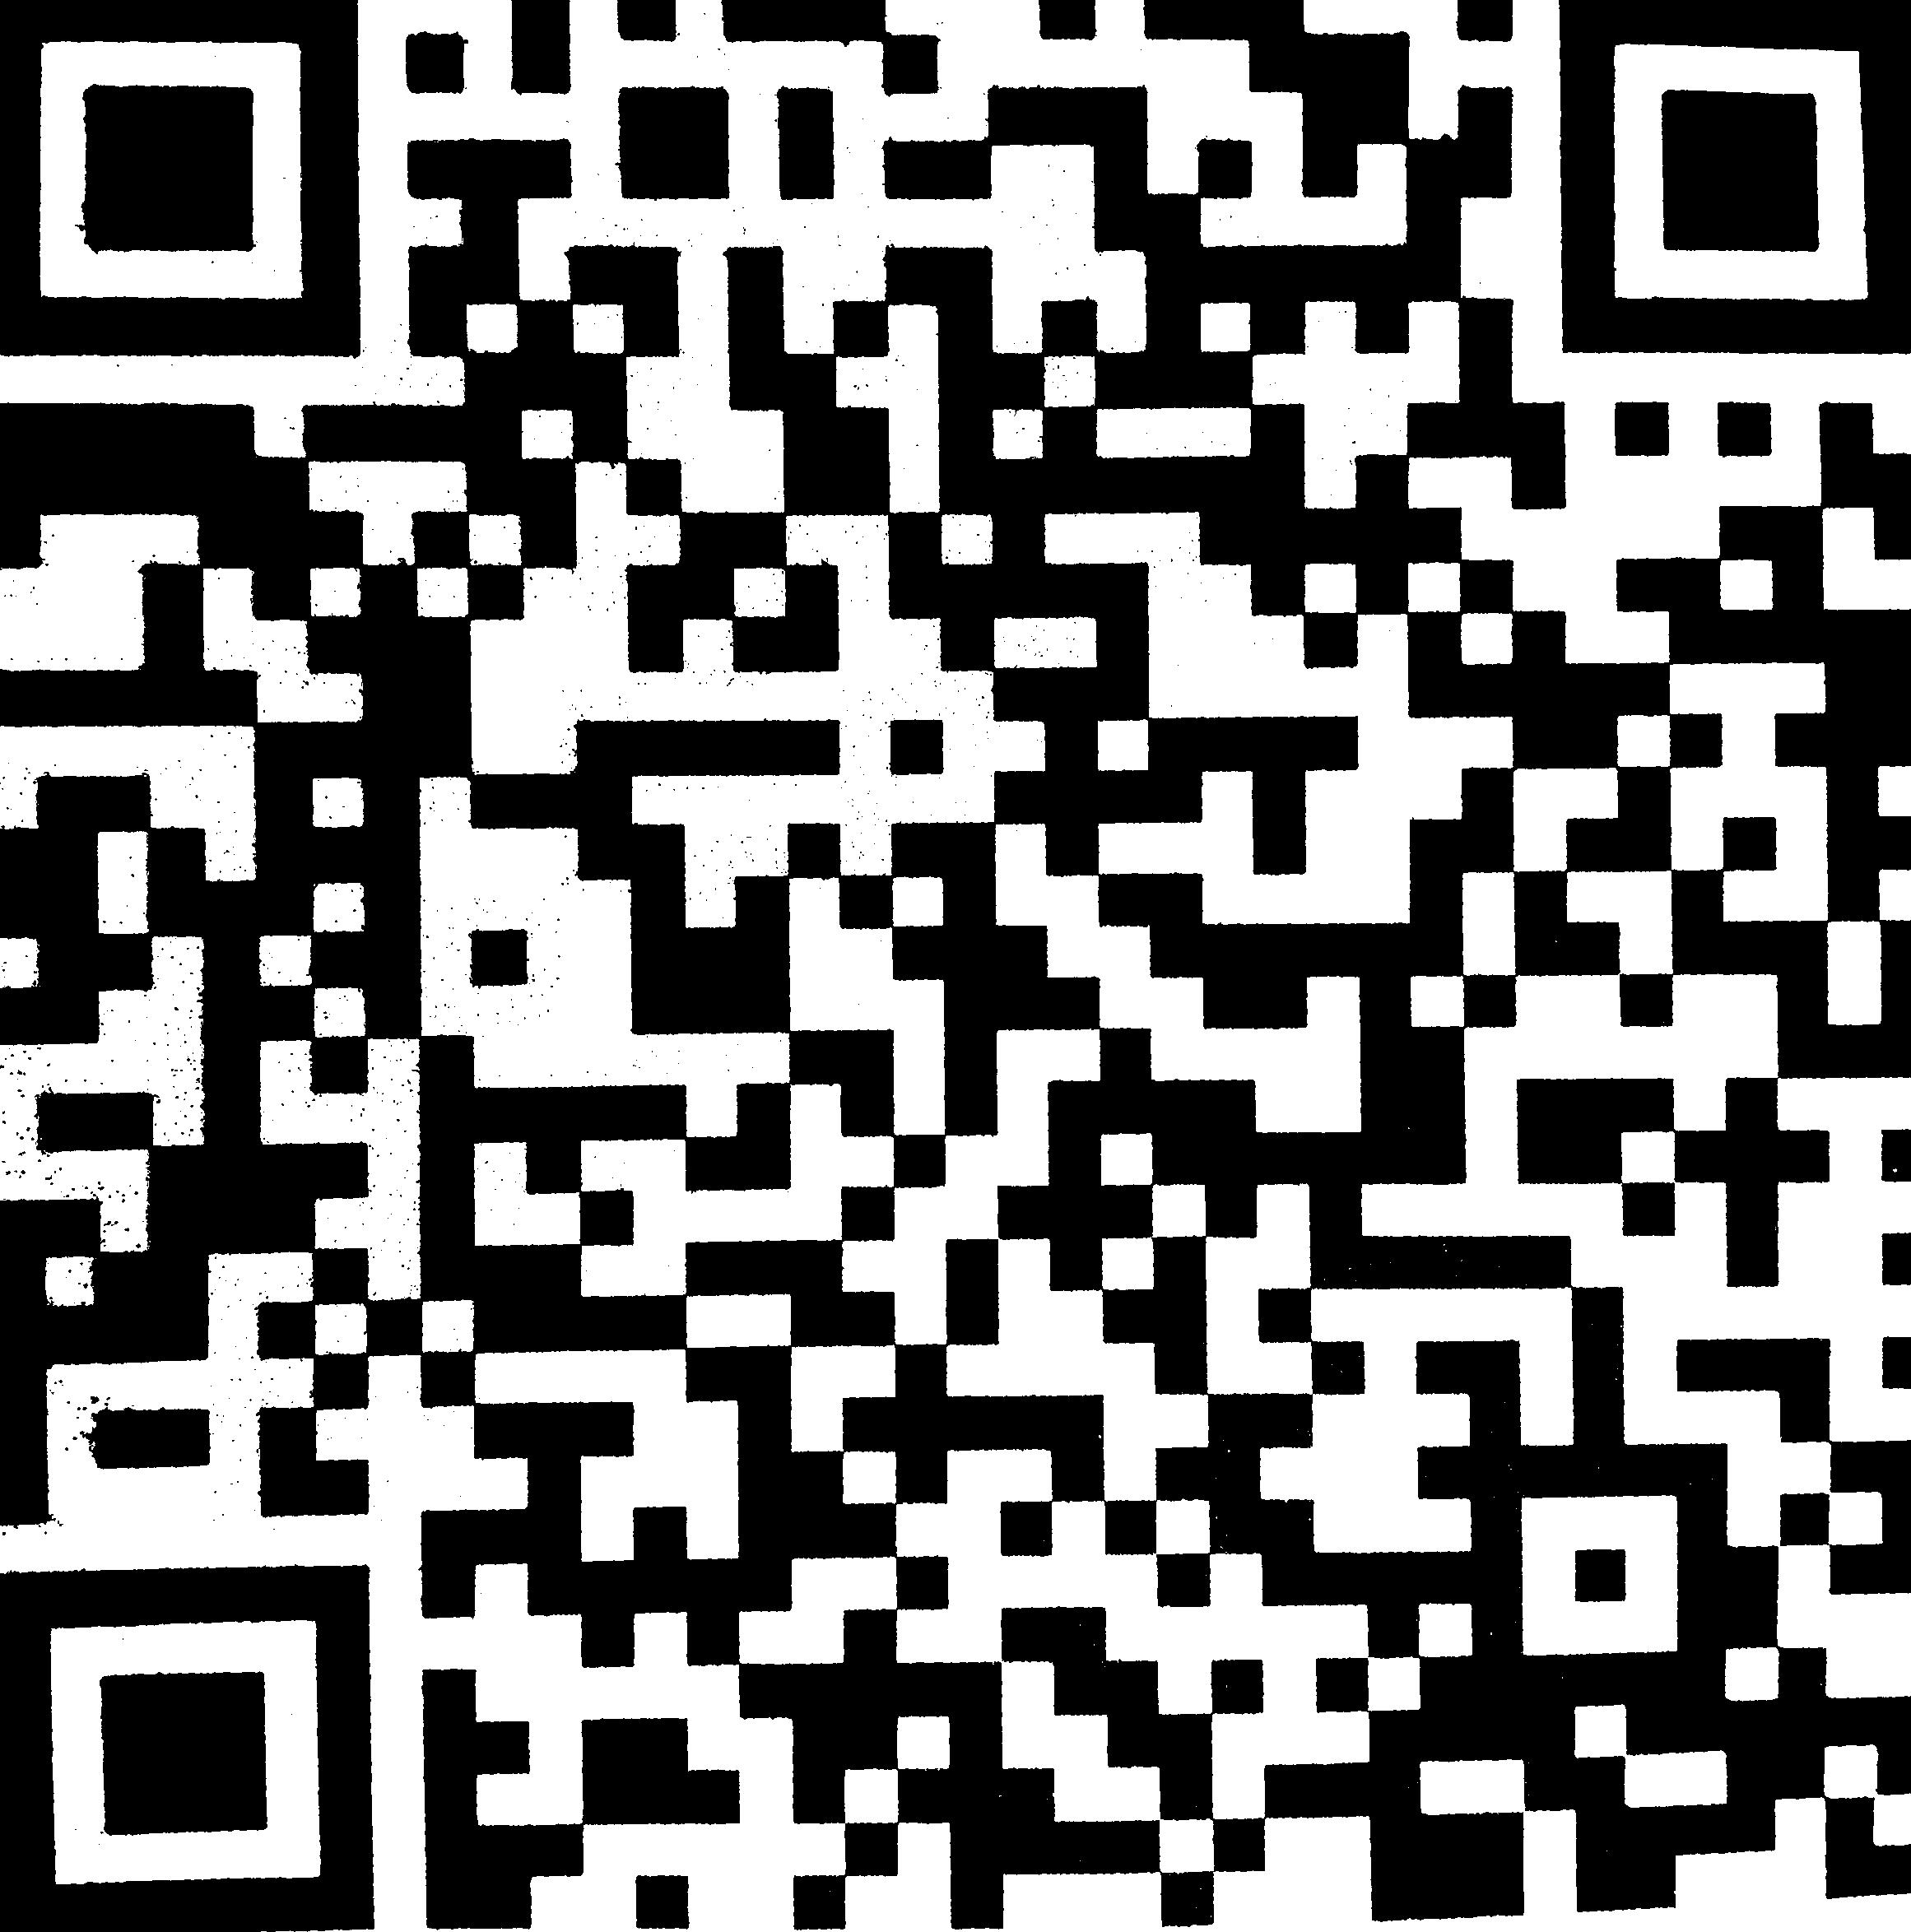
\includegraphics[width=3.68cm]{imagem16-LF}}\hfill
\subfloat[]{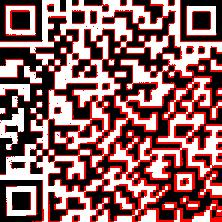
\includegraphics[width=3.68cm]{imagem16-LF-diff}}\\
\subfloat[]{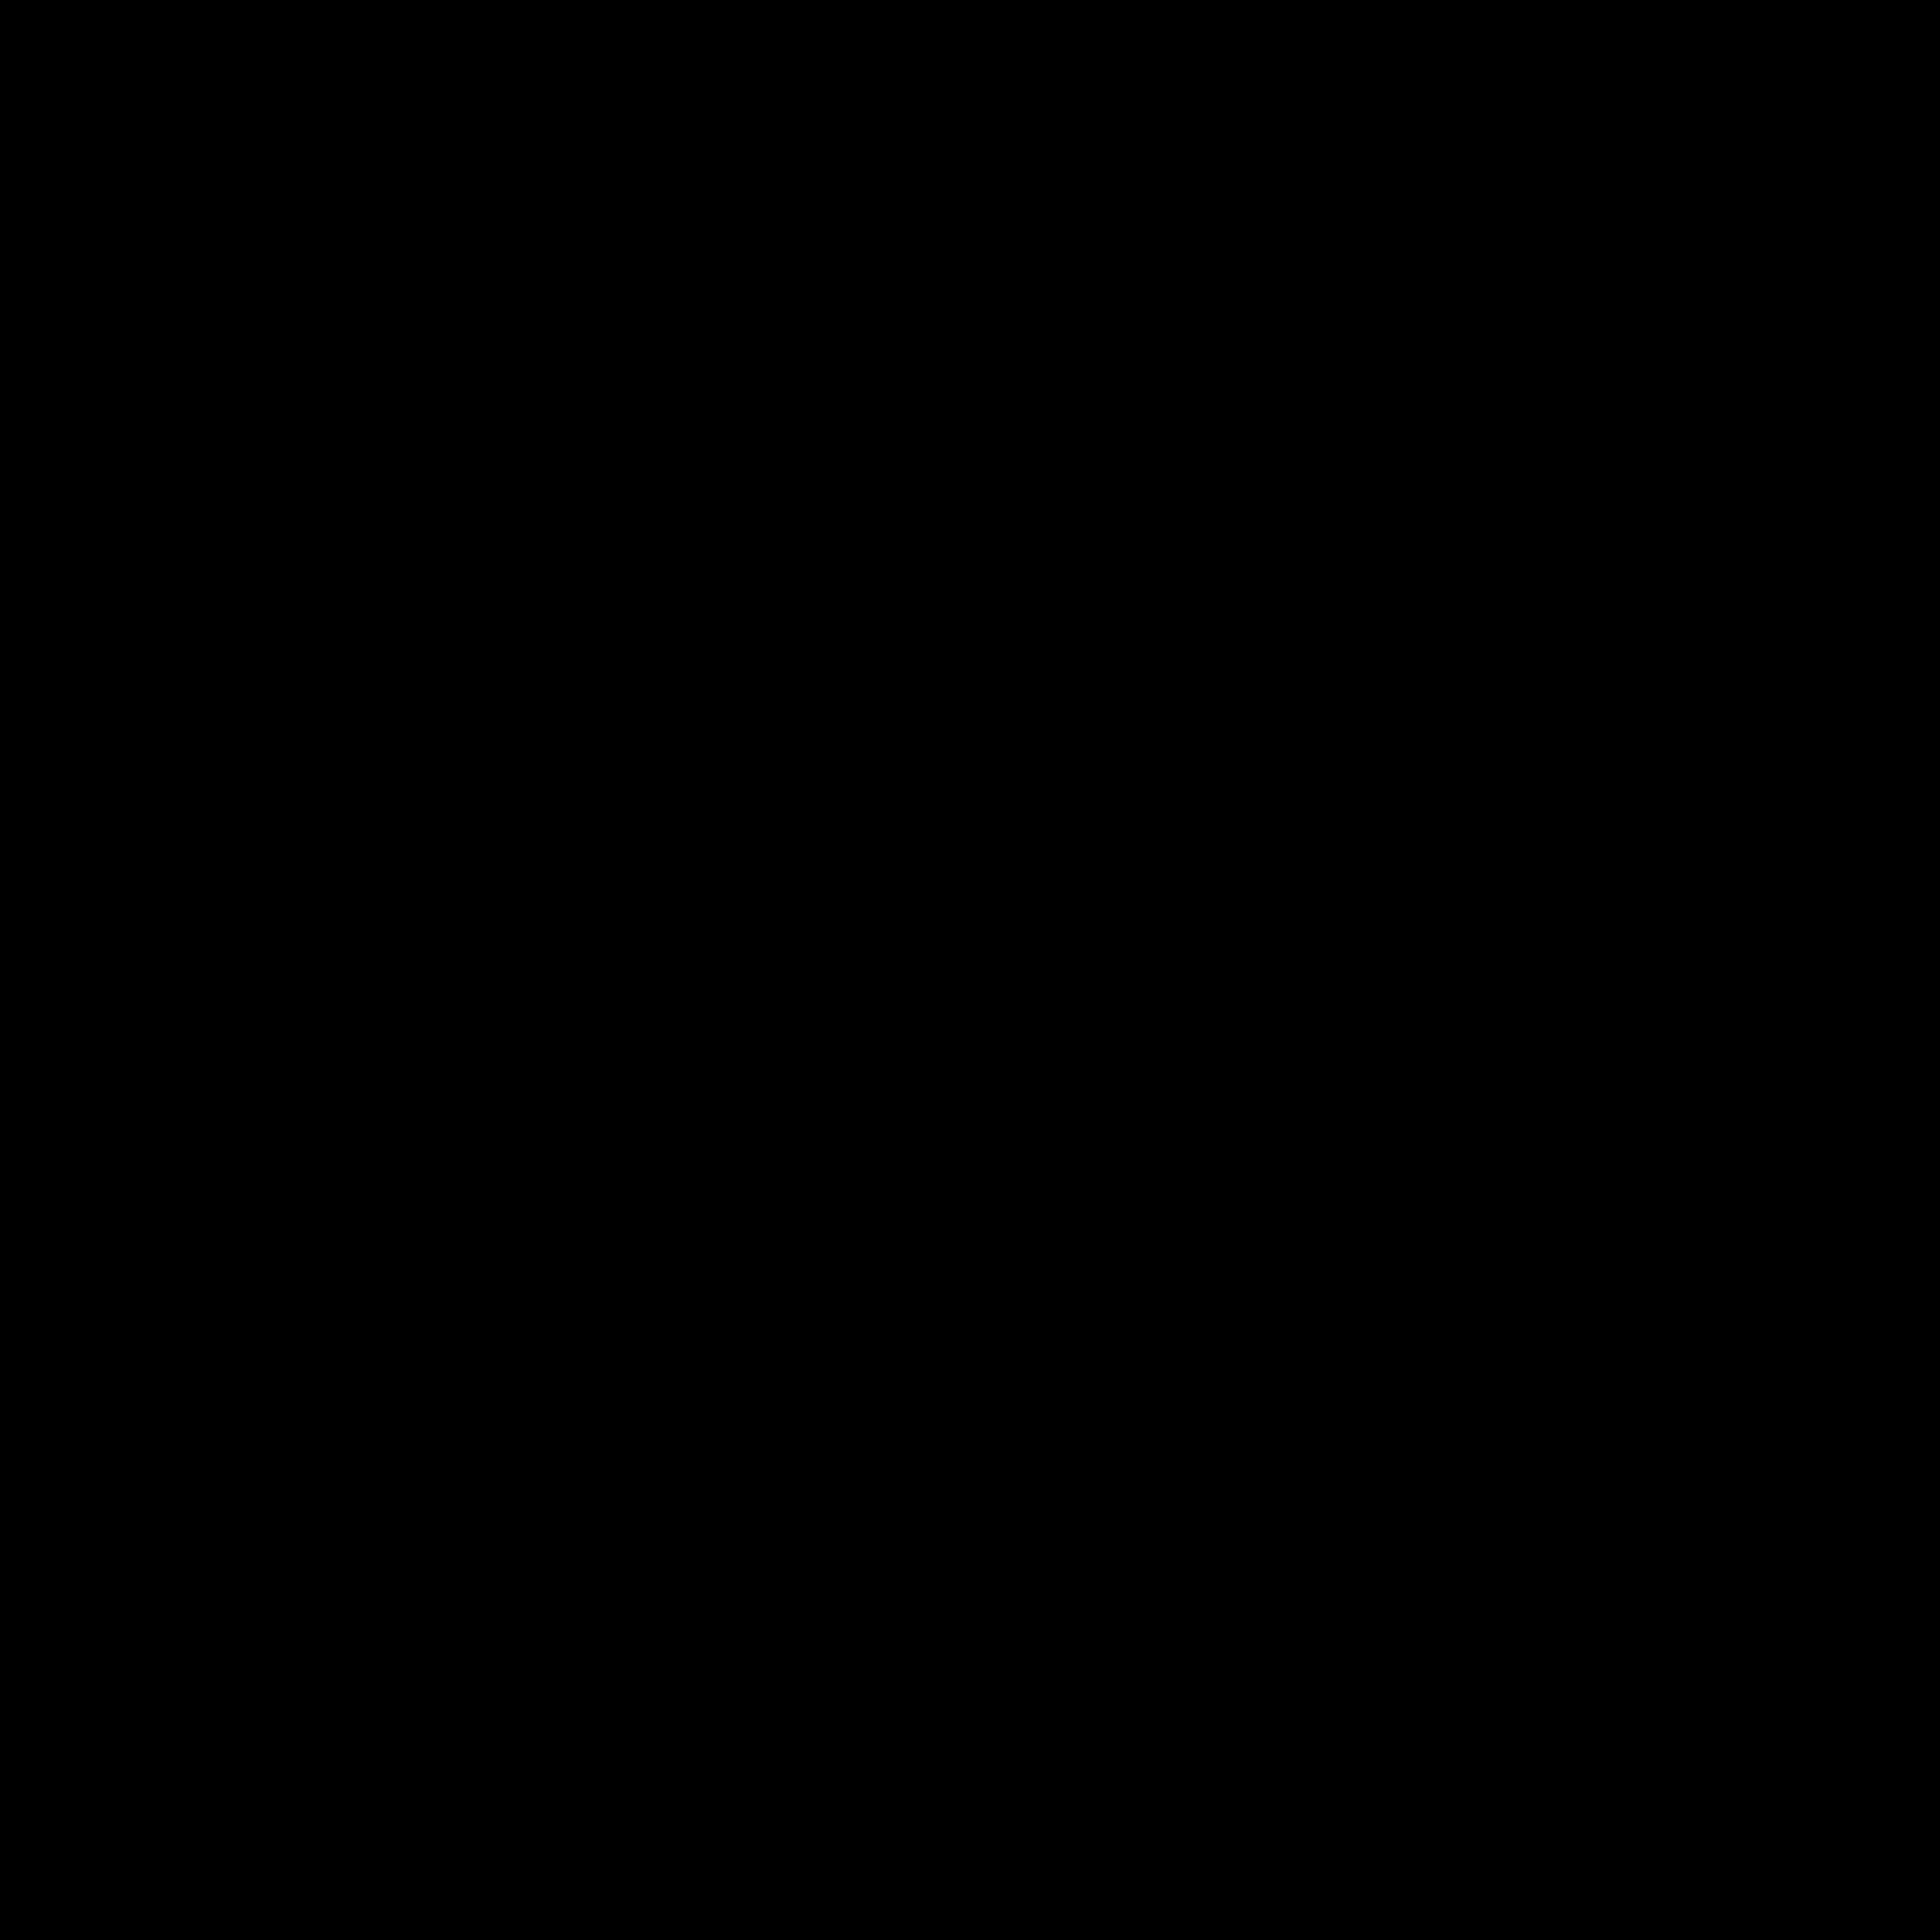
\includegraphics[width=3.68cm]{imagem29-LF}} \hfill 
\subfloat[]{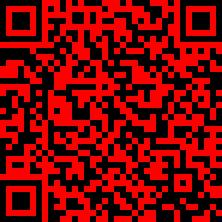
\includegraphics[width=3.68cm]{imagem29-LF-diff}}
\vspace{-0.1cm}
\caption{Imagens resultantes da Binarização com Limiar Fixo para o QR Code 3 nos padrões de (a) Iluminação 1, (c) Iluminação 2 e (e) Iluminação 3, com suas respectivas imagens diferença em (b), (d) e (f).} \label{figLF}
\end{minipage}

\vspace{0.4cm}
\noindent apresenta o resultado obtido com a utilização da técnica EH ao mesmo QR Code das Figuras 4 e 5, para assim facilitar a comparação entre os métodos, já que se trata das mesmas imagens.

De acordo com Gonzalez e Woods \cite{gonzales}, a equalização de histograma tem como objetivo redistribuir os valores de níveis de cinza do píxeis, de forma a obter uma melhora no contraste da imagem. Dessa modo, a equalização da imagem resultará em uma intensidade média $M$ distinta, a qual pode adequar-se melhor ou não aos propósitos da binarização. Na Figura \ref{imagemEH}, observa-se o espalhamento das barras do histograma sobre a escala de cinza após a equalização, para a qual é utlizada a imagem do QR Code 1 no padrão de Iluminação 2, na qual a técnica \emph{EH} obteve melhor resultado, evidenciado na Tabela \ref{tabP2}.

\subsection{Binarização em Sub-Regiões (S)} \label{Cdiv} 
O último método proposto neste artigo consiste em, primeiramente, subdividir a imagem em $n$ sub-regiões retangulares, assim cada uma é binarizada separadamente utilizando a intensidade média $M$ como limiar.
Neste artigo escolheu-se $n=9$, para o qual observa-se os resultados na Figura \ref{figS}. 


\hspace{-0.38cm}
\begin{minipage}[b]{\columnwidth}
\captionsetup{type=figure}
\subfloat[]{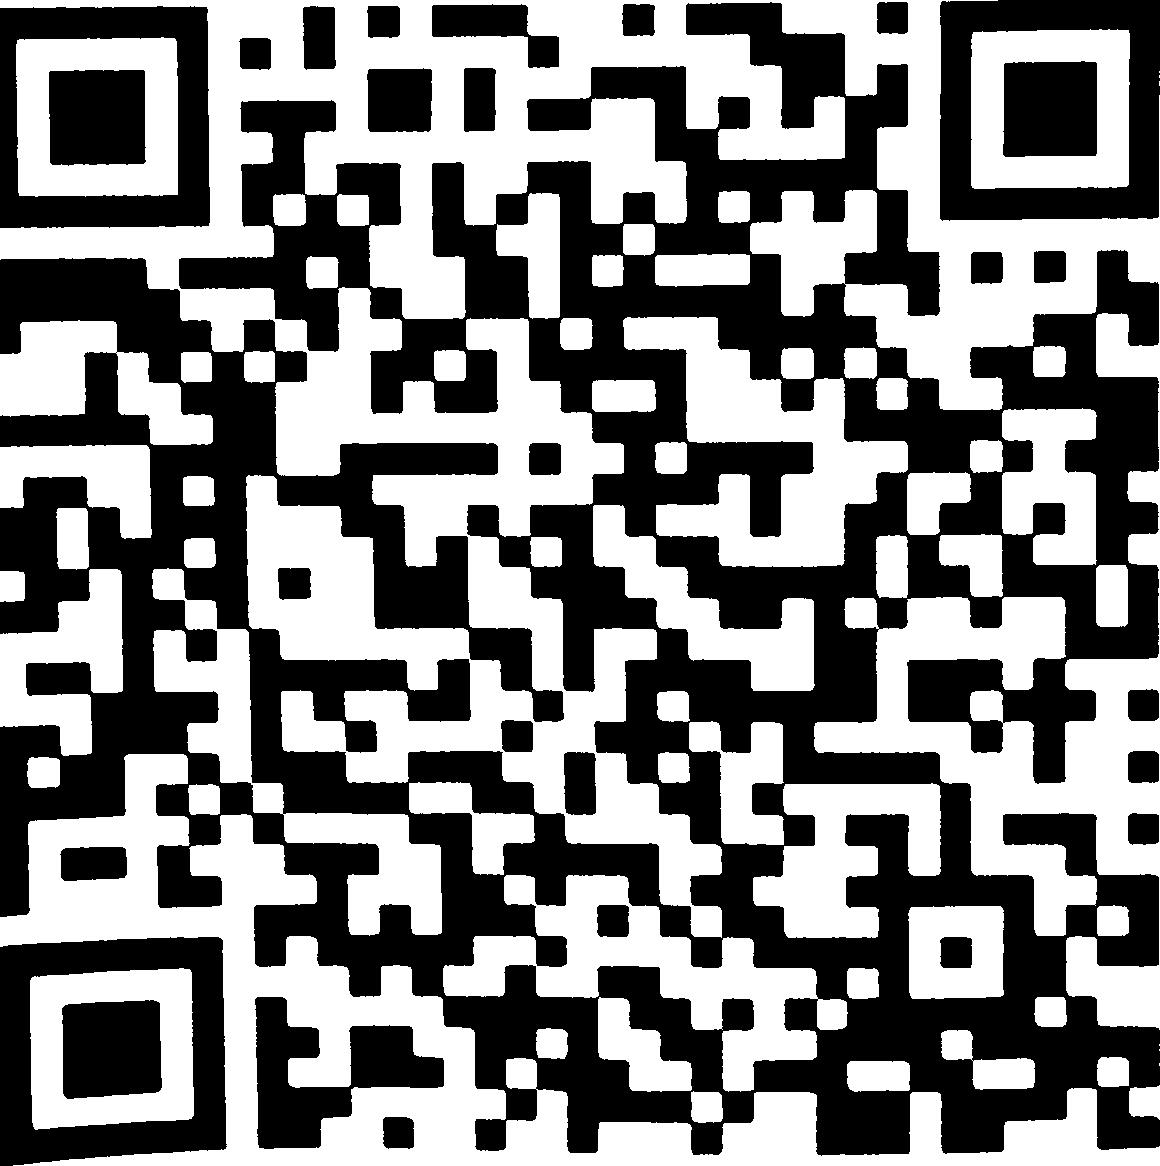
\includegraphics[width=3.68cm]{imagem03-LV}} \hfill
\subfloat[]{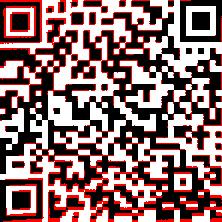
\includegraphics[width=3.68cm]{imagem03-LV-diff}} \\
\subfloat[]{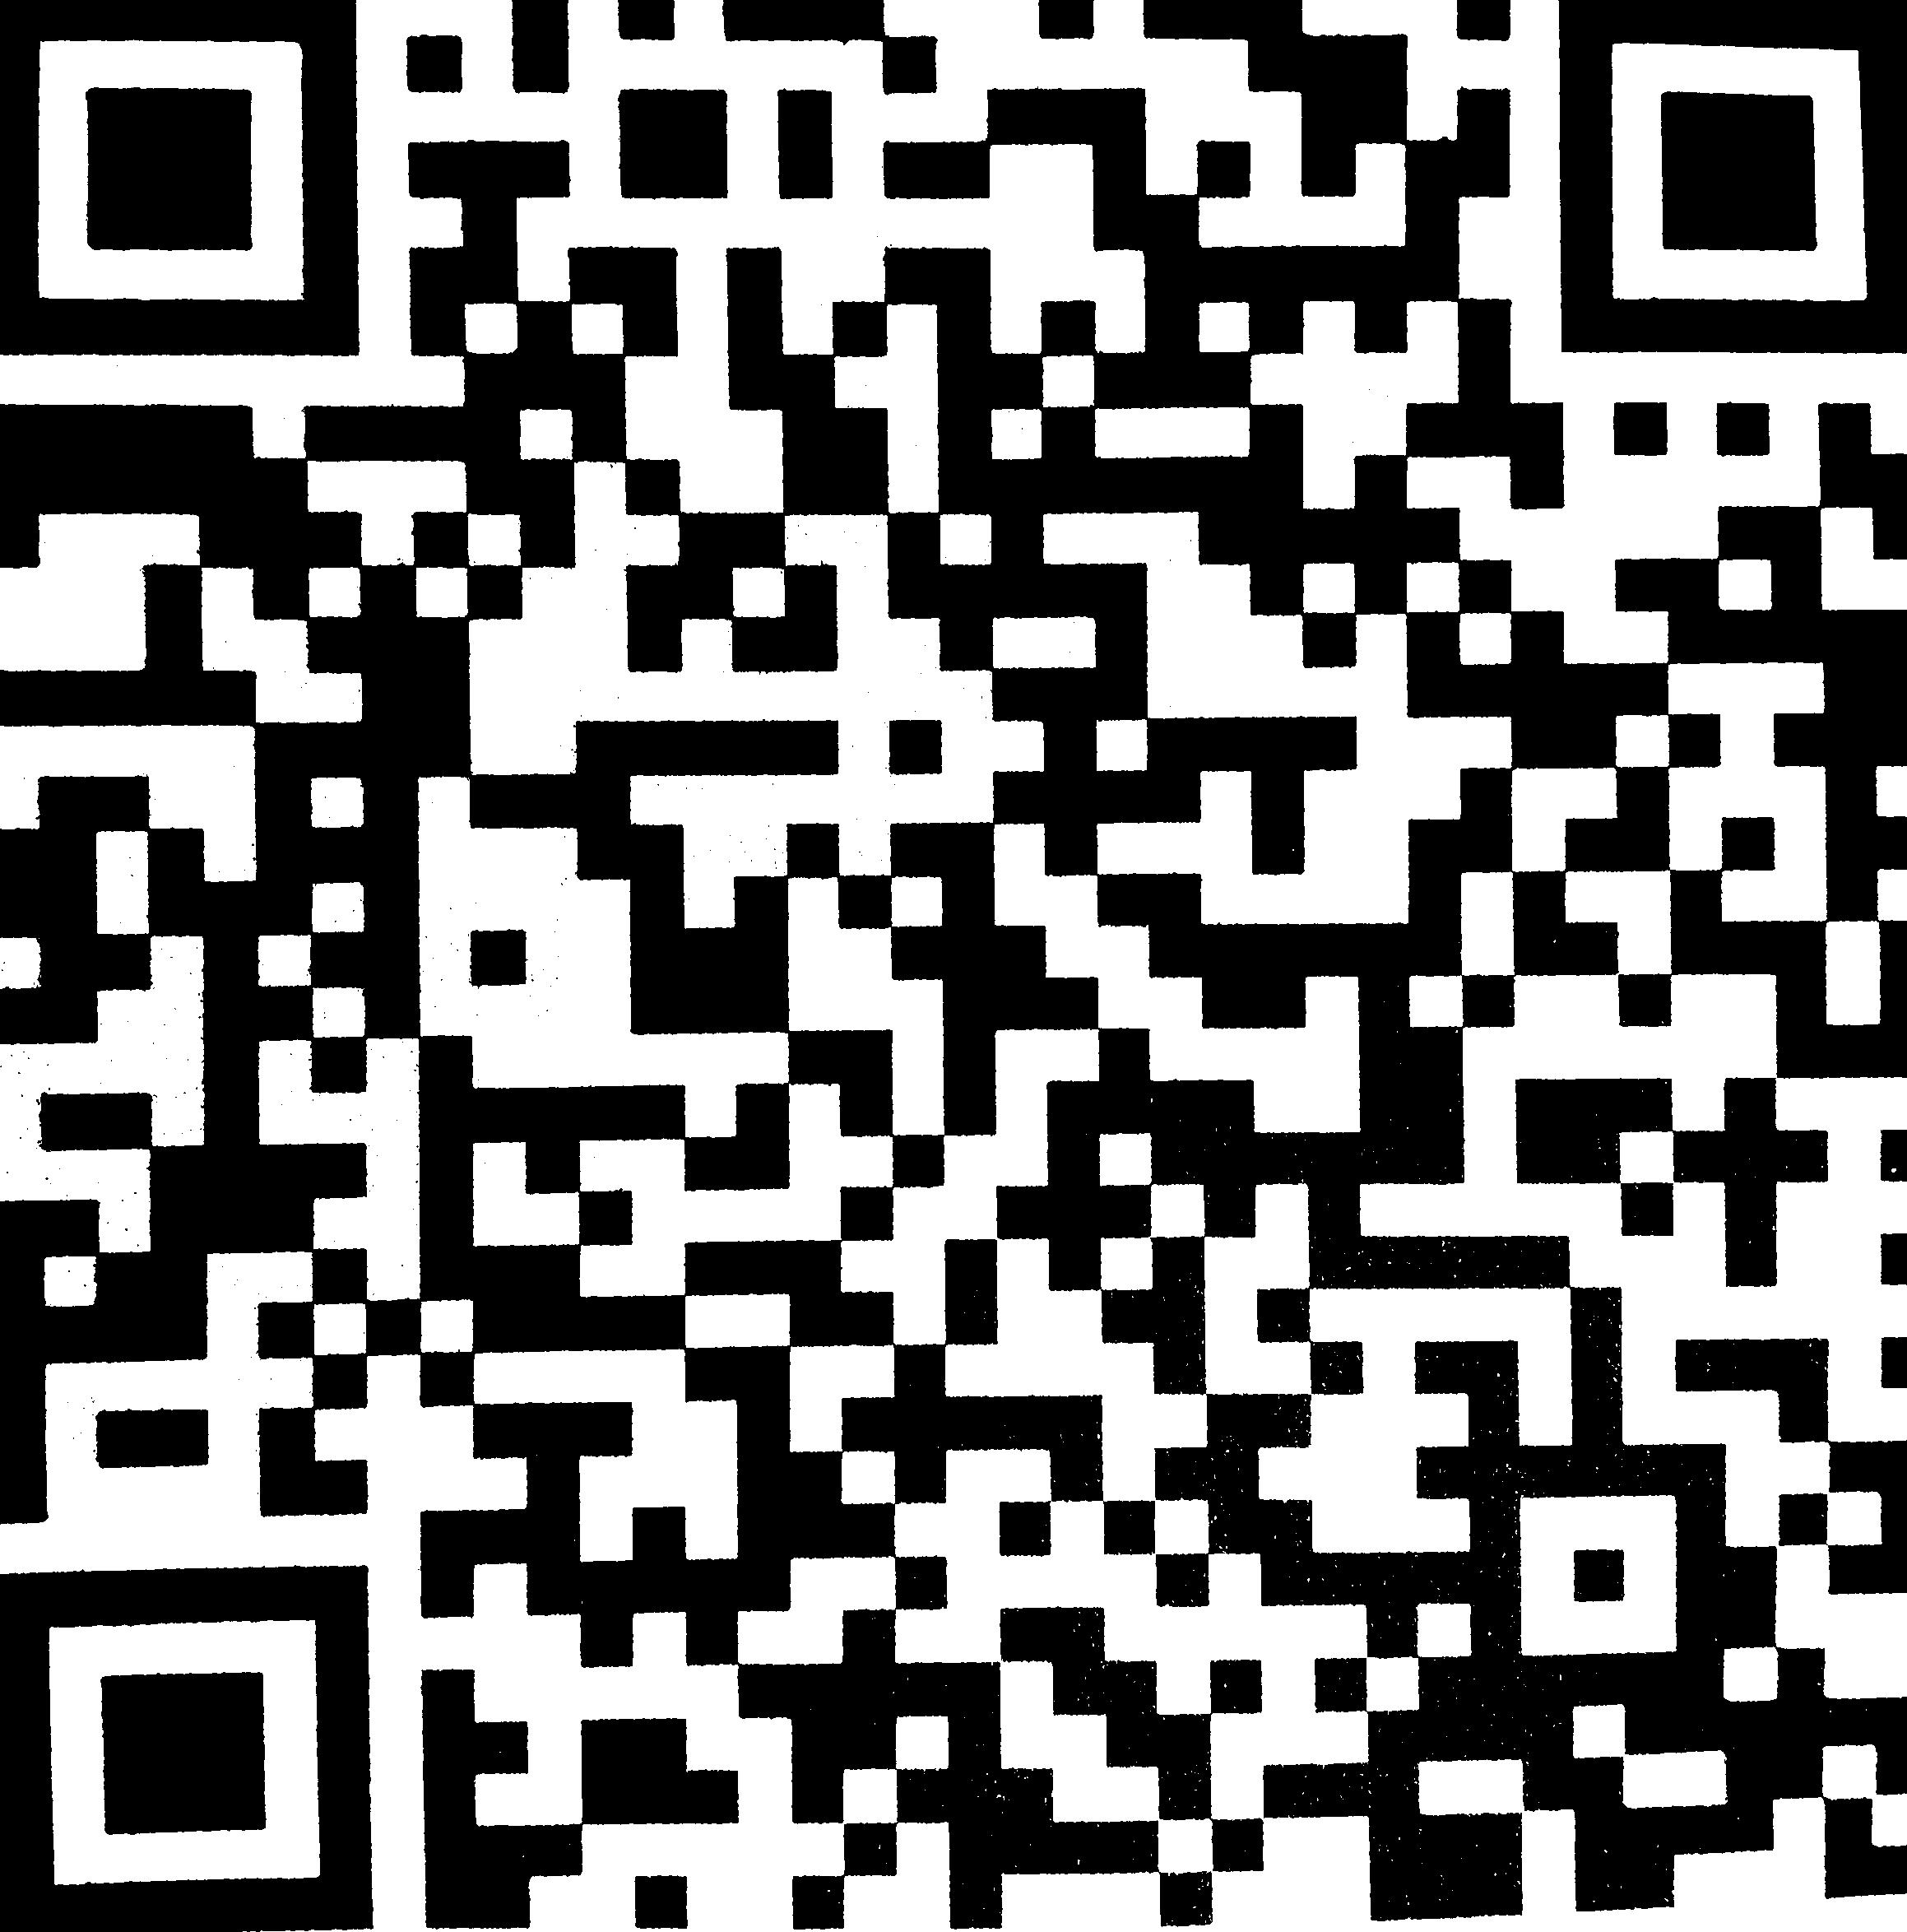
\includegraphics[width=3.68cm]{imagem16-LV}}\hfill
\subfloat[]{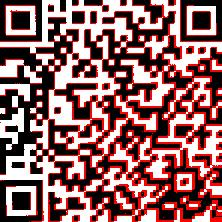
\includegraphics[width=3.68cm]{imagem16-LV-diff}}\\
\subfloat[]{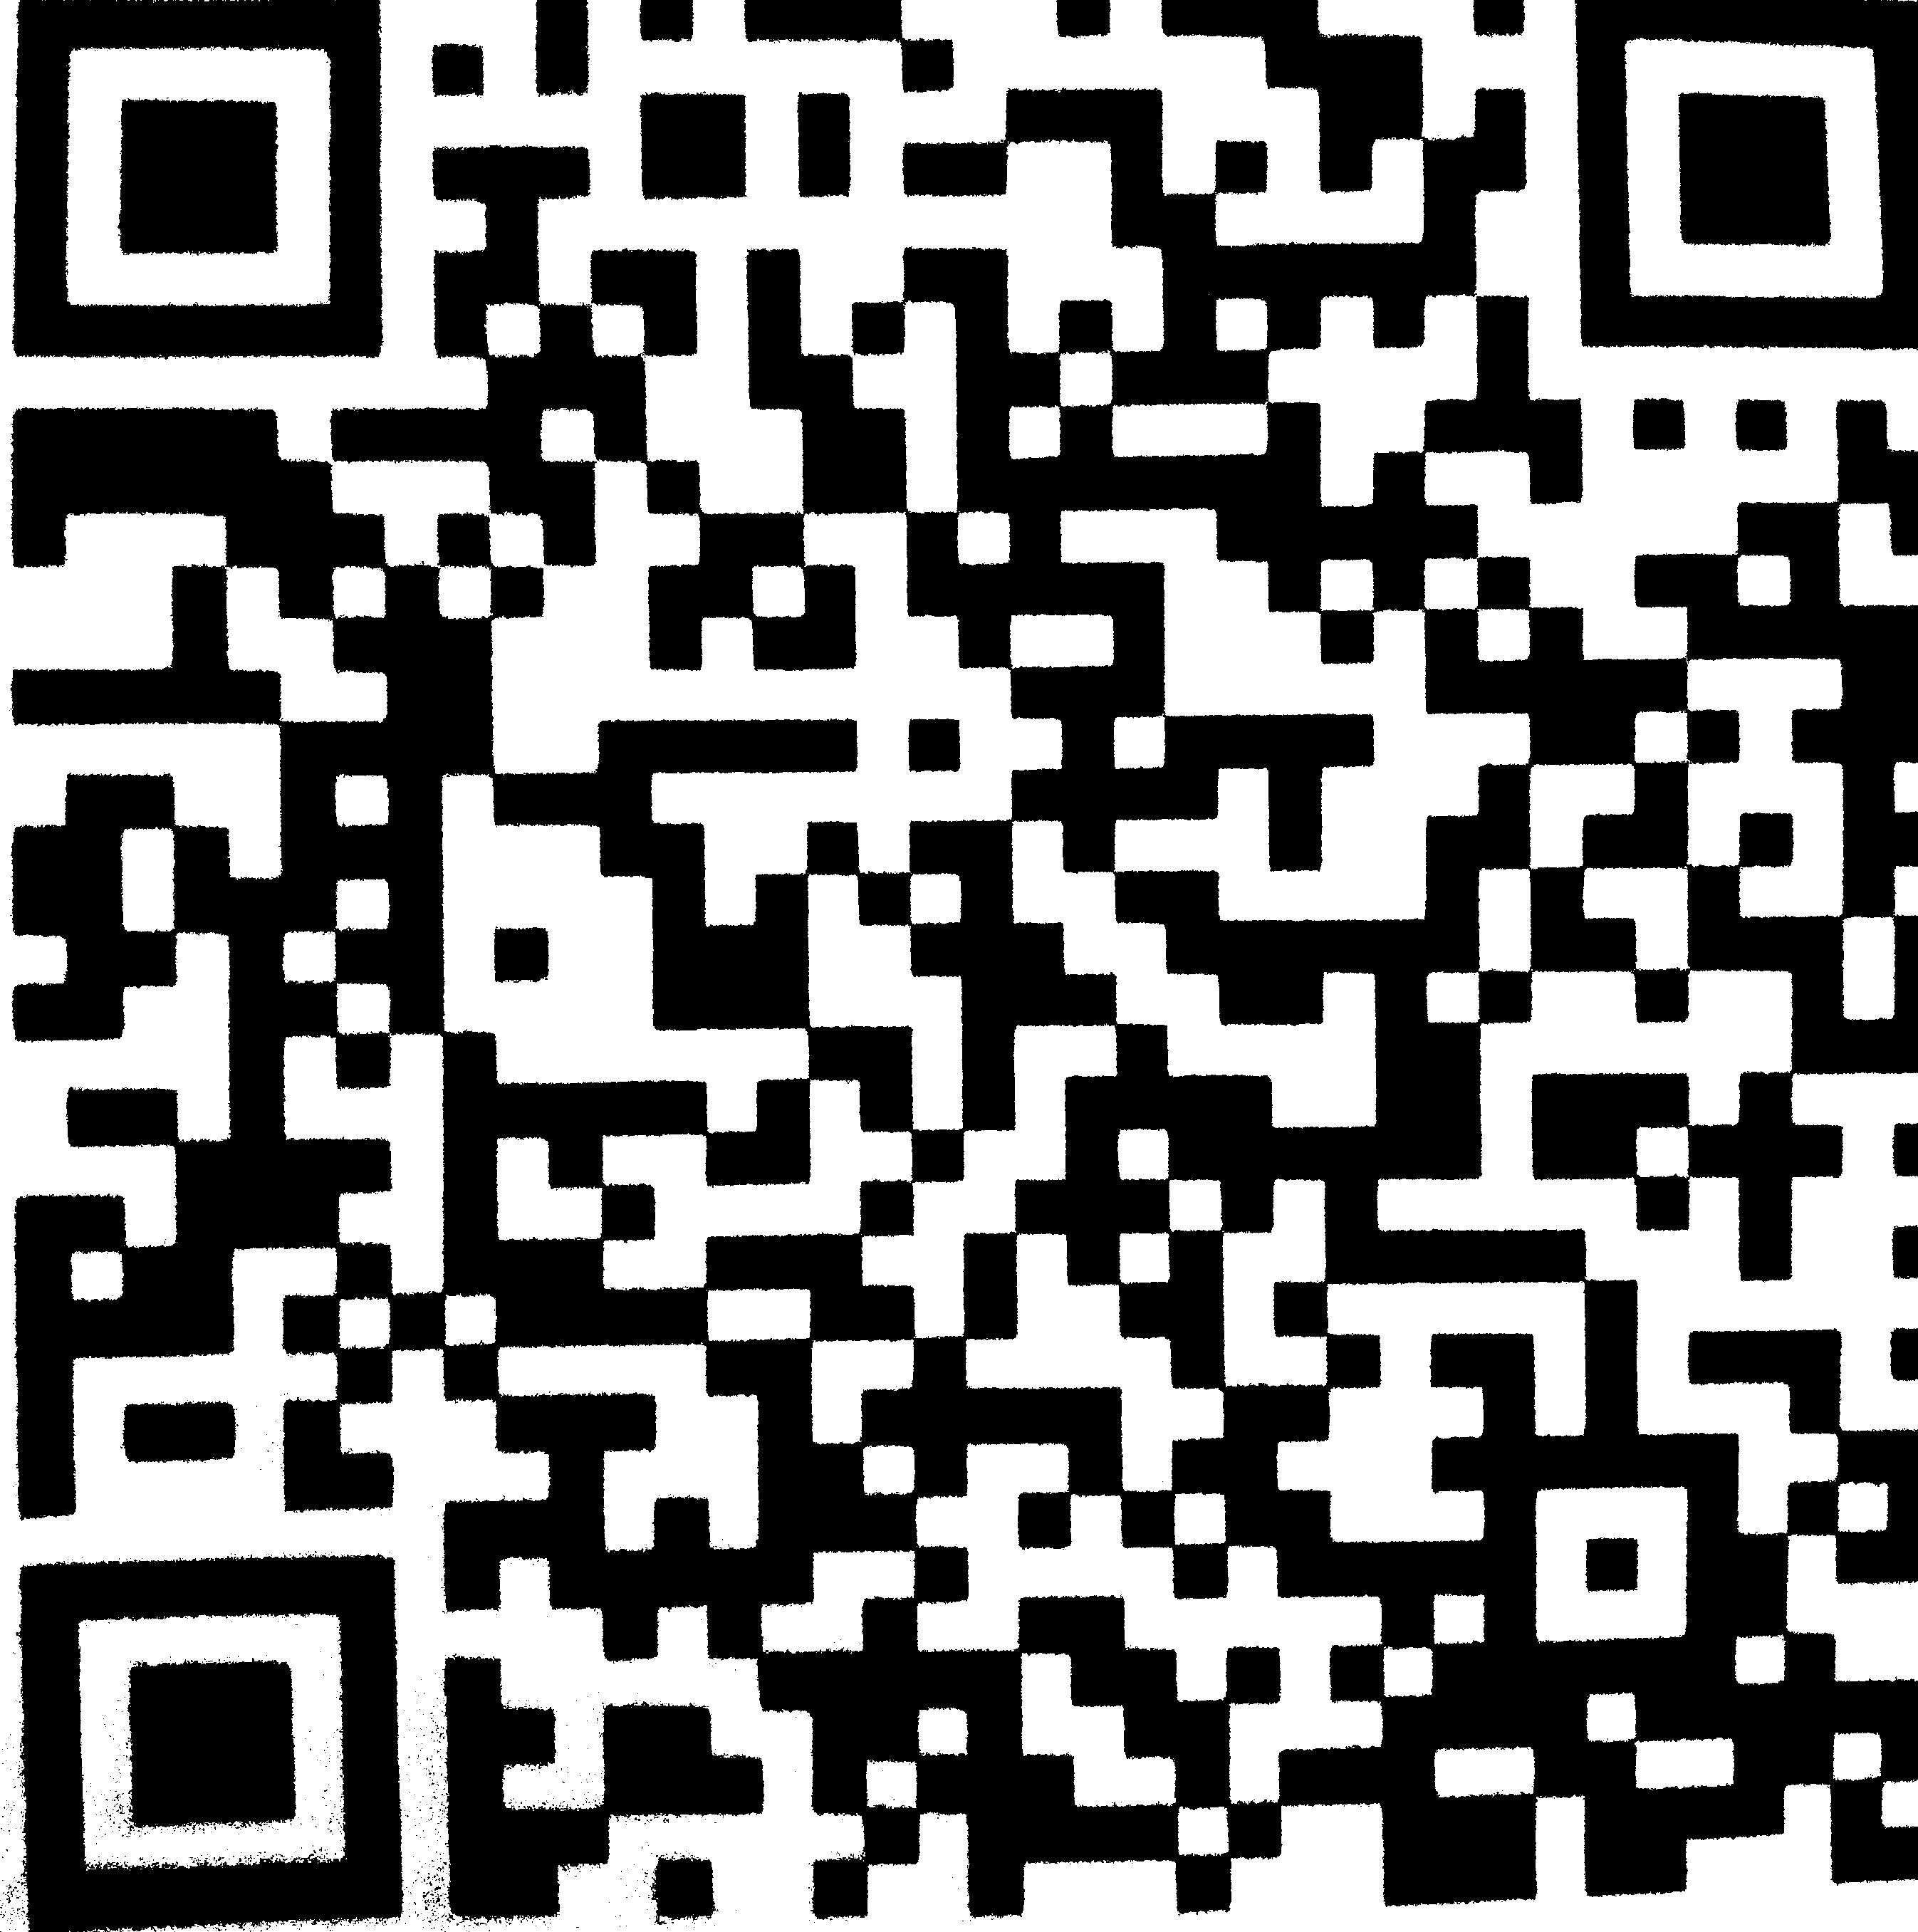
\includegraphics[width=3.68cm]{imagem29-LV}} \hfill 
\subfloat[]{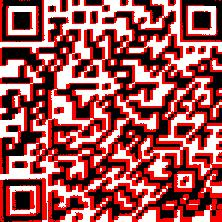
\includegraphics[width=3.68cm]{imagem29-LV-diff}}
\vspace{-0.1cm}
\caption{Imagens resultantes da Binarização com Limiar Variável para o QR Code 3 nos padrões de (a) Iluminação 1, (c) Iluminação 2 e (e) Iluminação 3, com suas respectivas imagens diferença em (b), (d) e (f).} \label{figLV}
\end{minipage}

%\vspace{0.05cm}
\hspace{-0.38cm}
\begin{minipage}{\columnwidth}
\captionsetup{type=figure}
\subfloat[]{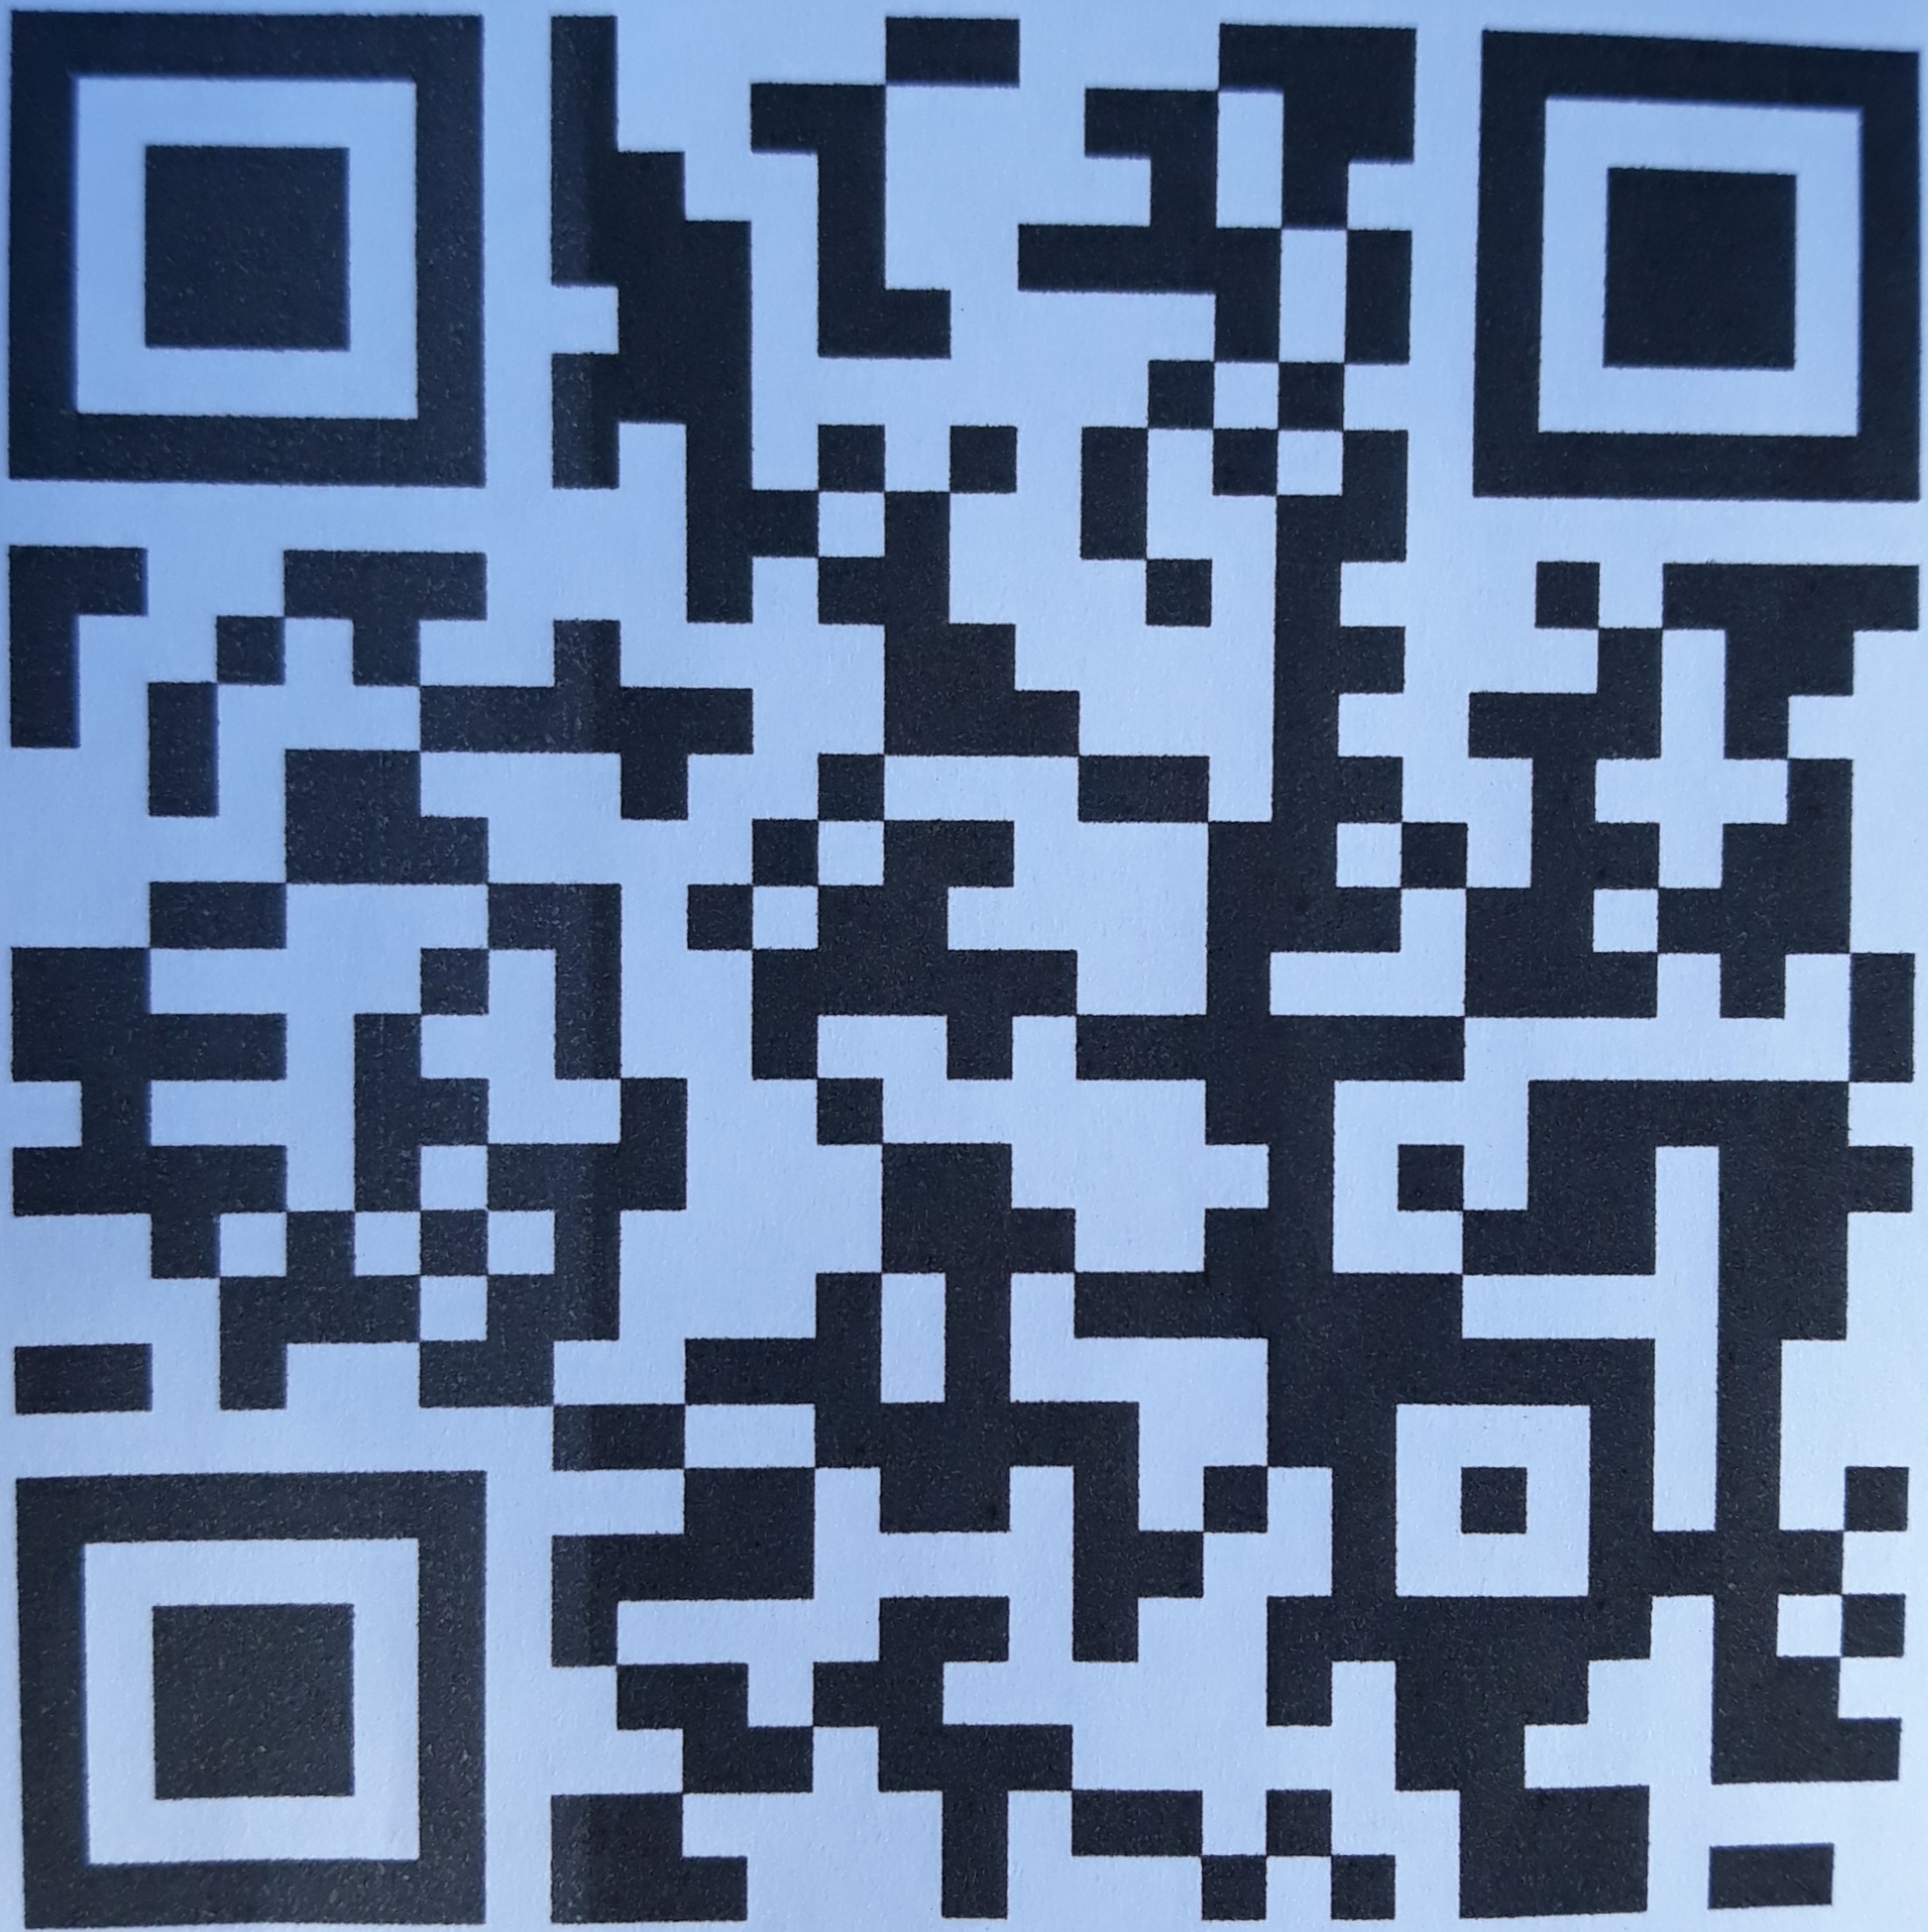
\includegraphics[width=3.5cm]{imagem14}}\hfill
\subfloat[]{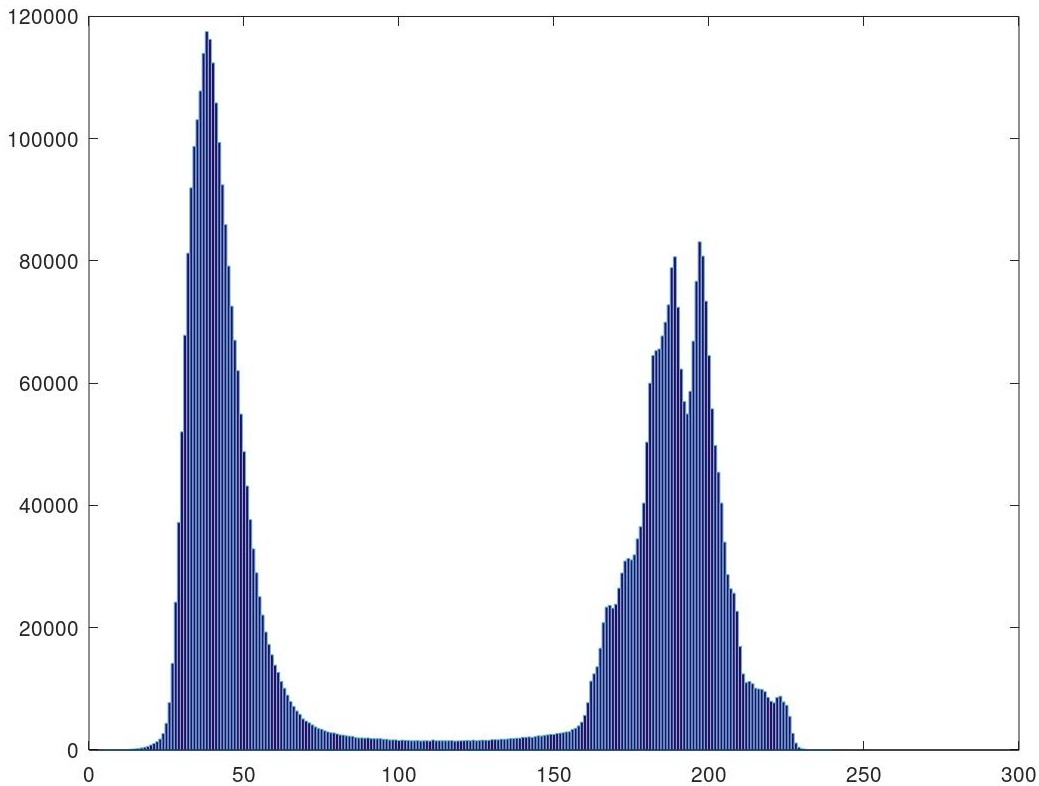
\includegraphics[width=4.52cm]{imagem14-hist}}\\
\subfloat[]{
\includegraphics[width=3.5cm]{imagem14-EH-primaria}}\hfill 
\subfloat[]{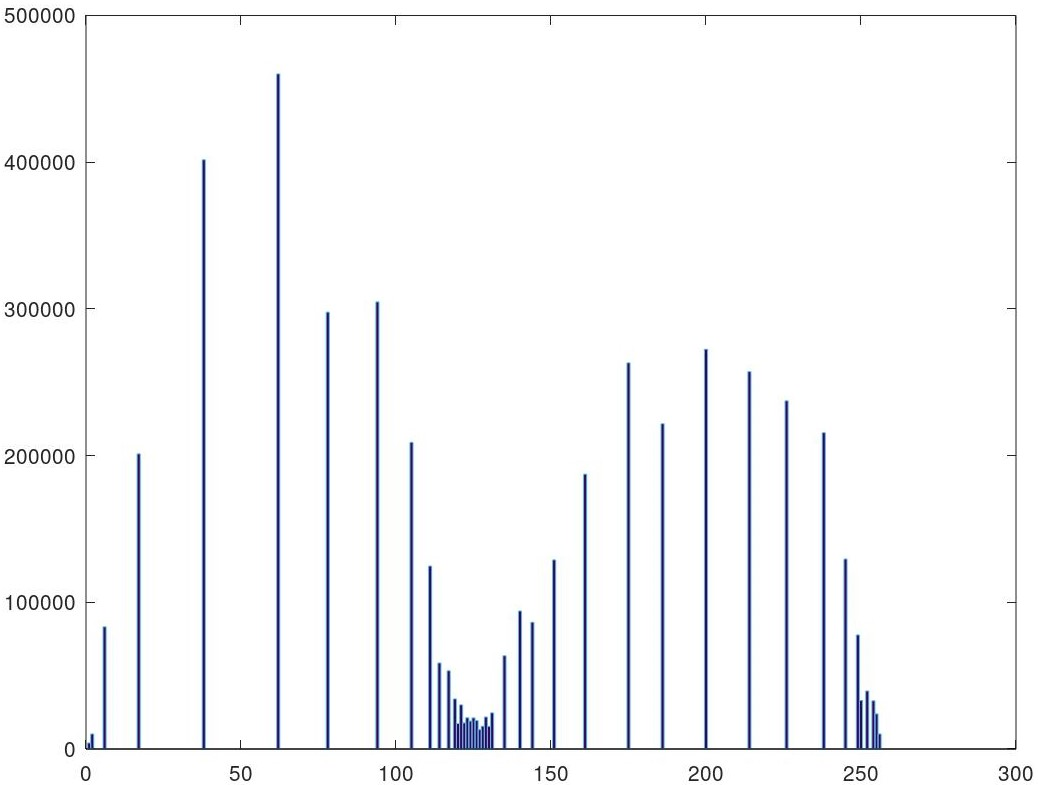
\includegraphics[width=4.52cm]{imagem14-EH-hist}} 
\vspace{-0.1cm}
\caption{(a) QR Code 1 submetido ao padrão de Iluminação 2, (b) histograma de (a), (c) imagem resultante da equalização de histograma e (d) histograma de (c).}
\label{imagemEH}
\end{minipage}


\hspace{-0.38cm}
\begin{minipage}[h]{\columnwidth}
\captionsetup{type=figure}
\subfloat[]{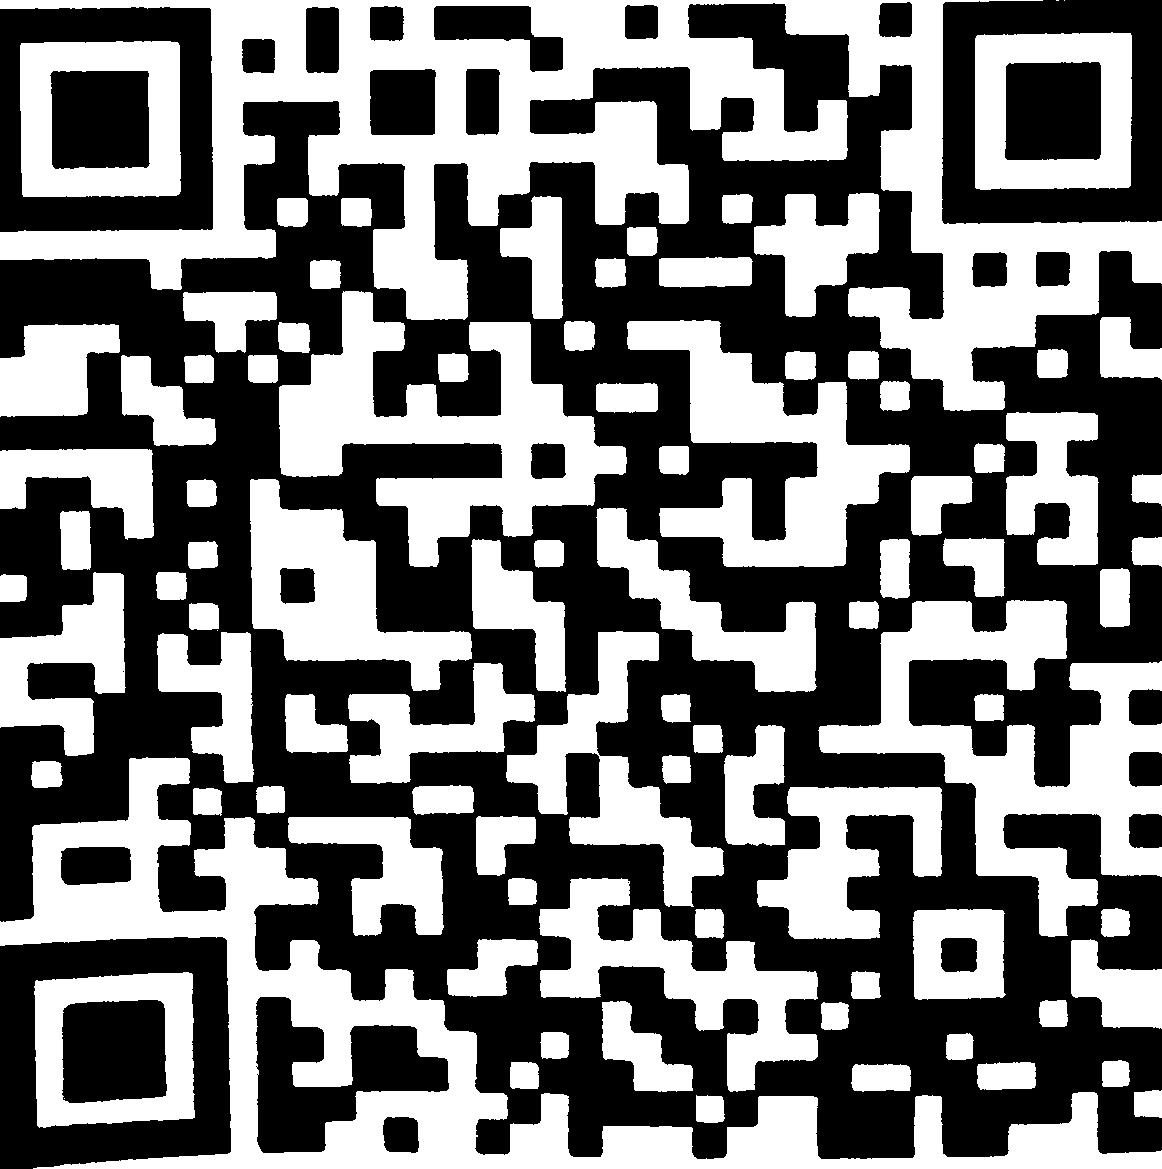
\includegraphics[width=3.68cm]{imagem03-EH}} \hfill
\subfloat[]{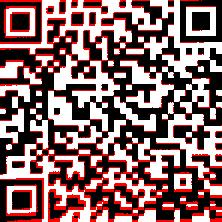
\includegraphics[width=3.68cm]{imagem03-EH-diff}} \\
\subfloat[]{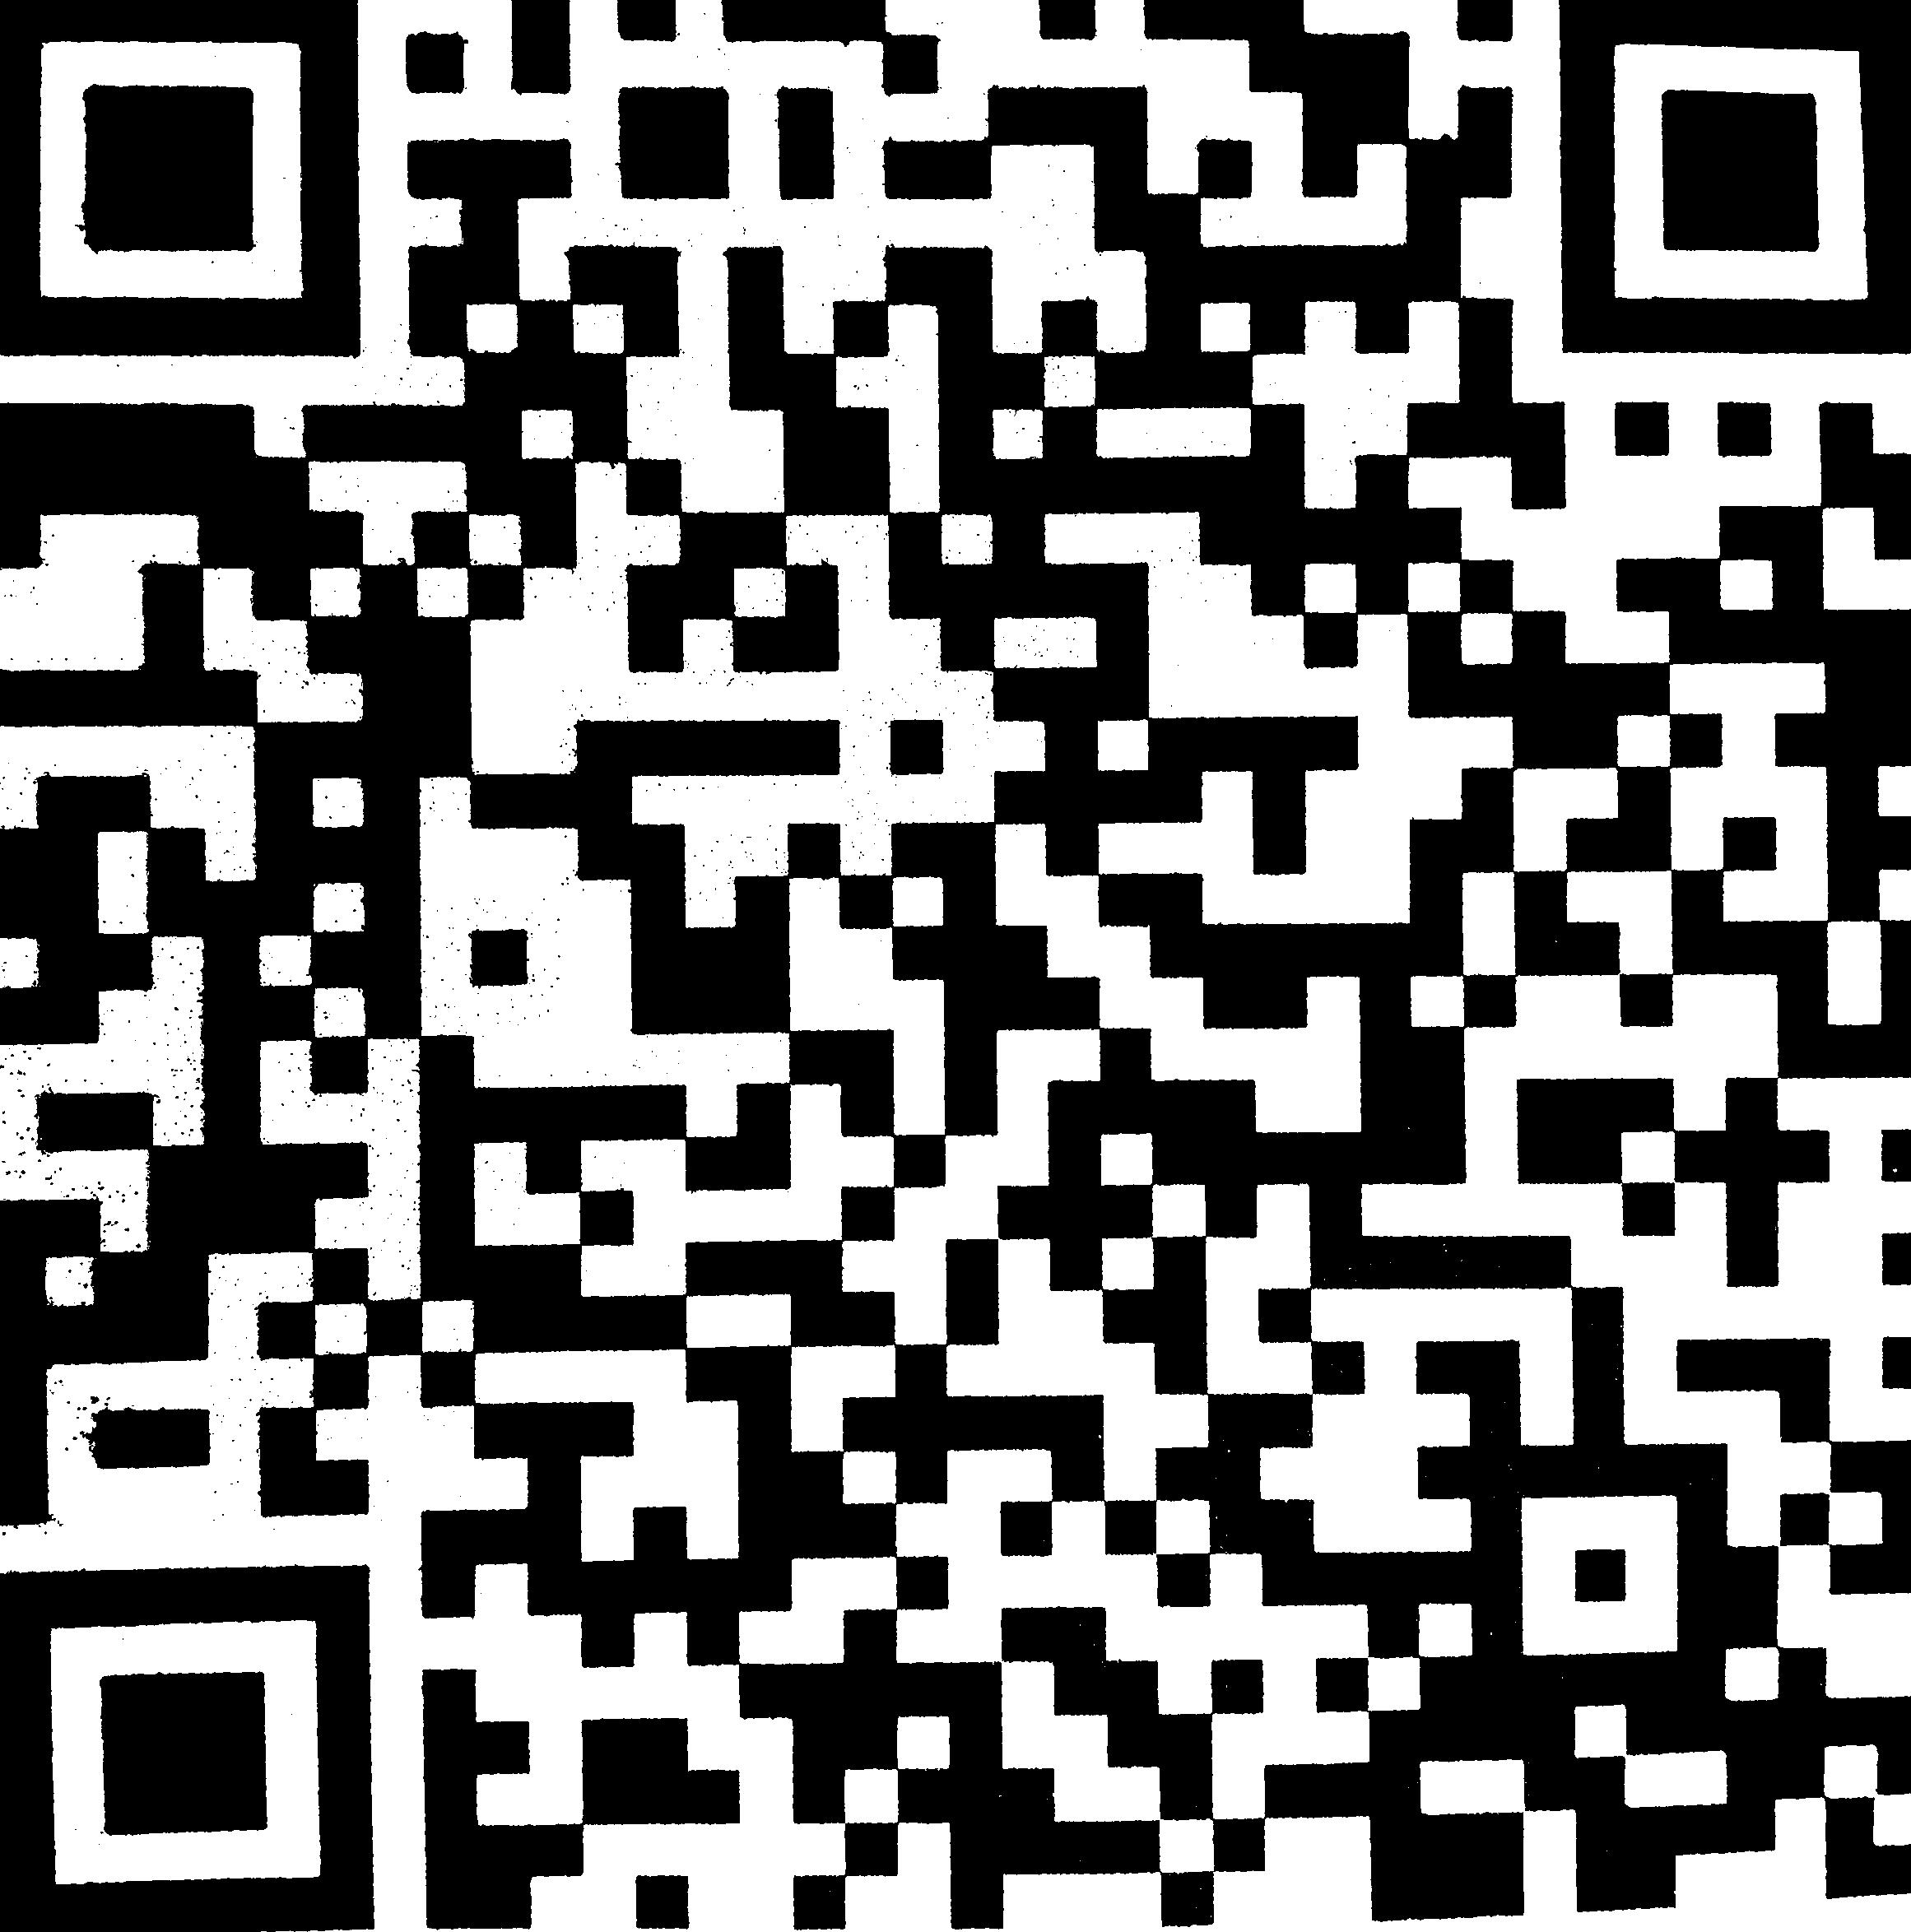
\includegraphics[width=3.68cm]{imagem16-EH}}\hfill
\subfloat[]{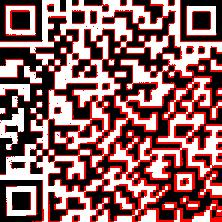
\includegraphics[width=3.68cm]{imagem16-EH-diff}}\\
\subfloat[]{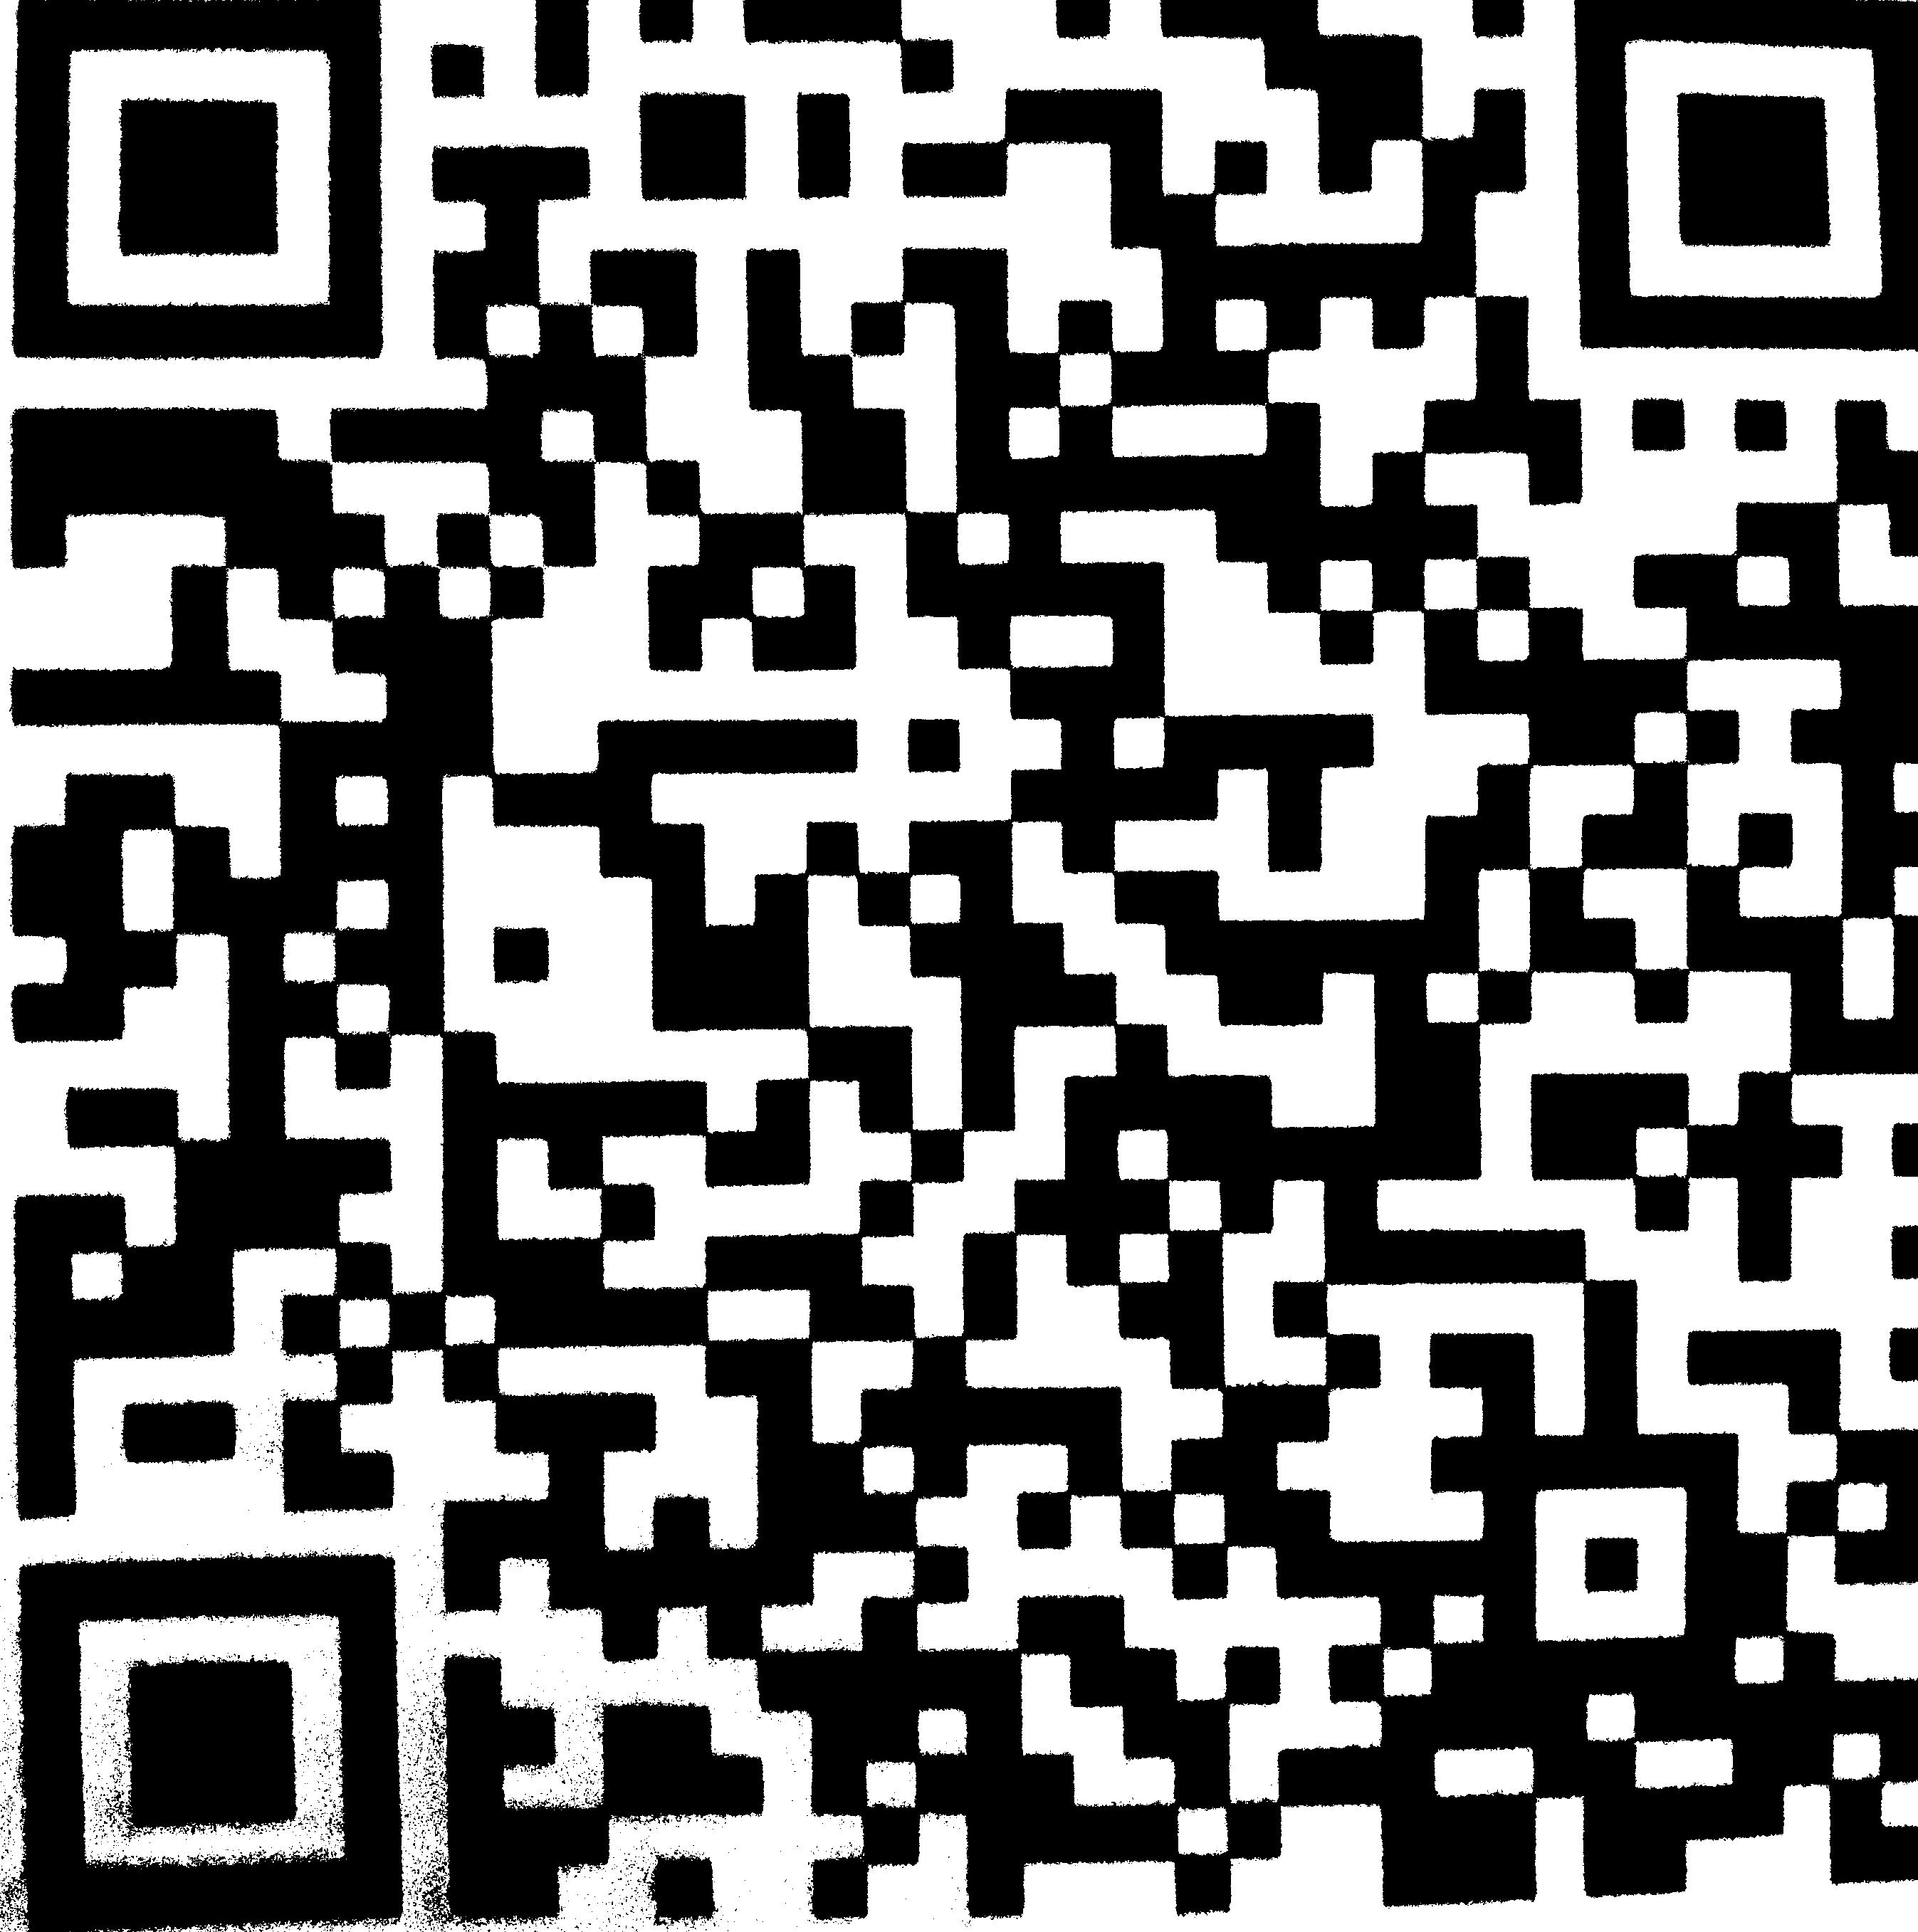
\includegraphics[width=3.68cm]{imagem29-EH}} \hfill
\subfloat[]{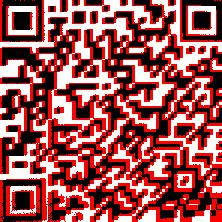
\includegraphics[width=3.68cm]{imagem29-EH-diff}}
\vspace{-0.1cm}
\caption{Imagens resultantes da Binarização Pós Equalização por Histograma para o QR Code 3 nos padrões de (a) Iluminação 1, (c) Iluminação 2 e (e) Iluminação 3, com suas respectivas imagens diferença em (b), (d) e (f).} \label{figEH}
\end{minipage}

\section{Análise dos resultados} \label{resultados}
Aplicando-se o processo descrito no fluxograma da Figura \ref{fluxograma} para as imagens coletadas obtém-se os resultados das Tabelas \ref{tabP1}, \ref{tabP2} e \ref{tabP3}, as quais informam os erros associados aos métodos aplicados e o método eficaz, ou seja que apresentou menor erro, para as imagens dos padrões de Iluminação 1, 2 e 3. 

A respeito dos métodos de binarização por limiar, há certa dificuldade em determinar qual métodos, \emph{LF} ou \emph{LV}, proporciona melhor resultado para uma determinada imagem, já que deve-se considerar que os píxeis pretos intrínsecos ao código afetam na determinação da intensidade média $M$, pois diminui seu maior numérico, ou seja, quanto maior o número de versão, maior será a quantidade de píxeis escuros instrínsecos ao código que influenciarão $M$. Para essas situações \emph{LF} pode ser método eficaz ou pelo menos superior a \emph{LV}, o que se confere nos resultados da Tabela \ref{tabP2} para as imagens de QR Codes de versões elevadas do padrão de Iluminação 2.

há uma dificuldade em determinar qual métodos, LF ou LV, gera um melhor resultado para uma determinada imagem.

Note também que analisando imagem a imagem, os valores percentuais de erro concentram-se em intervalos bem defini-\\


% imagem monocromatica = ou em escala de cinza
\hspace{-0.38cm}
\begin{minipage}[h]{\columnwidth}
\captionsetup{type=figure}
\subfloat[]{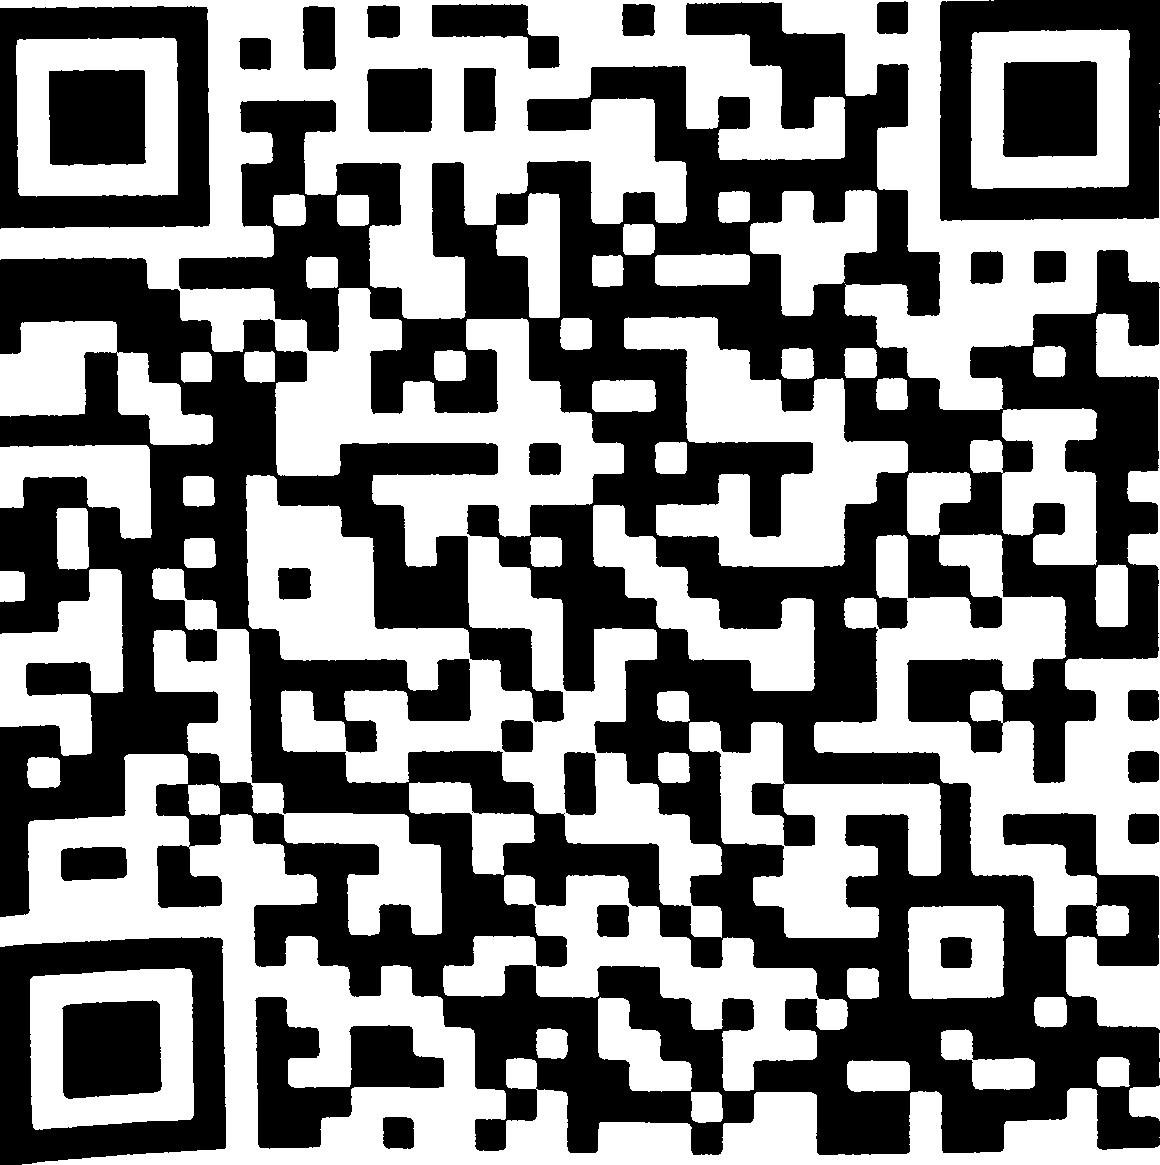
\includegraphics[width=3.68cm]{imagem03-S}}\hfill
\subfloat[]{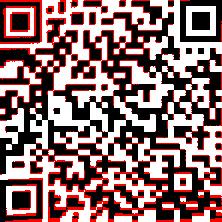
\includegraphics[width=3.68cm]{imagem03-S-diff}} \\
\subfloat[]{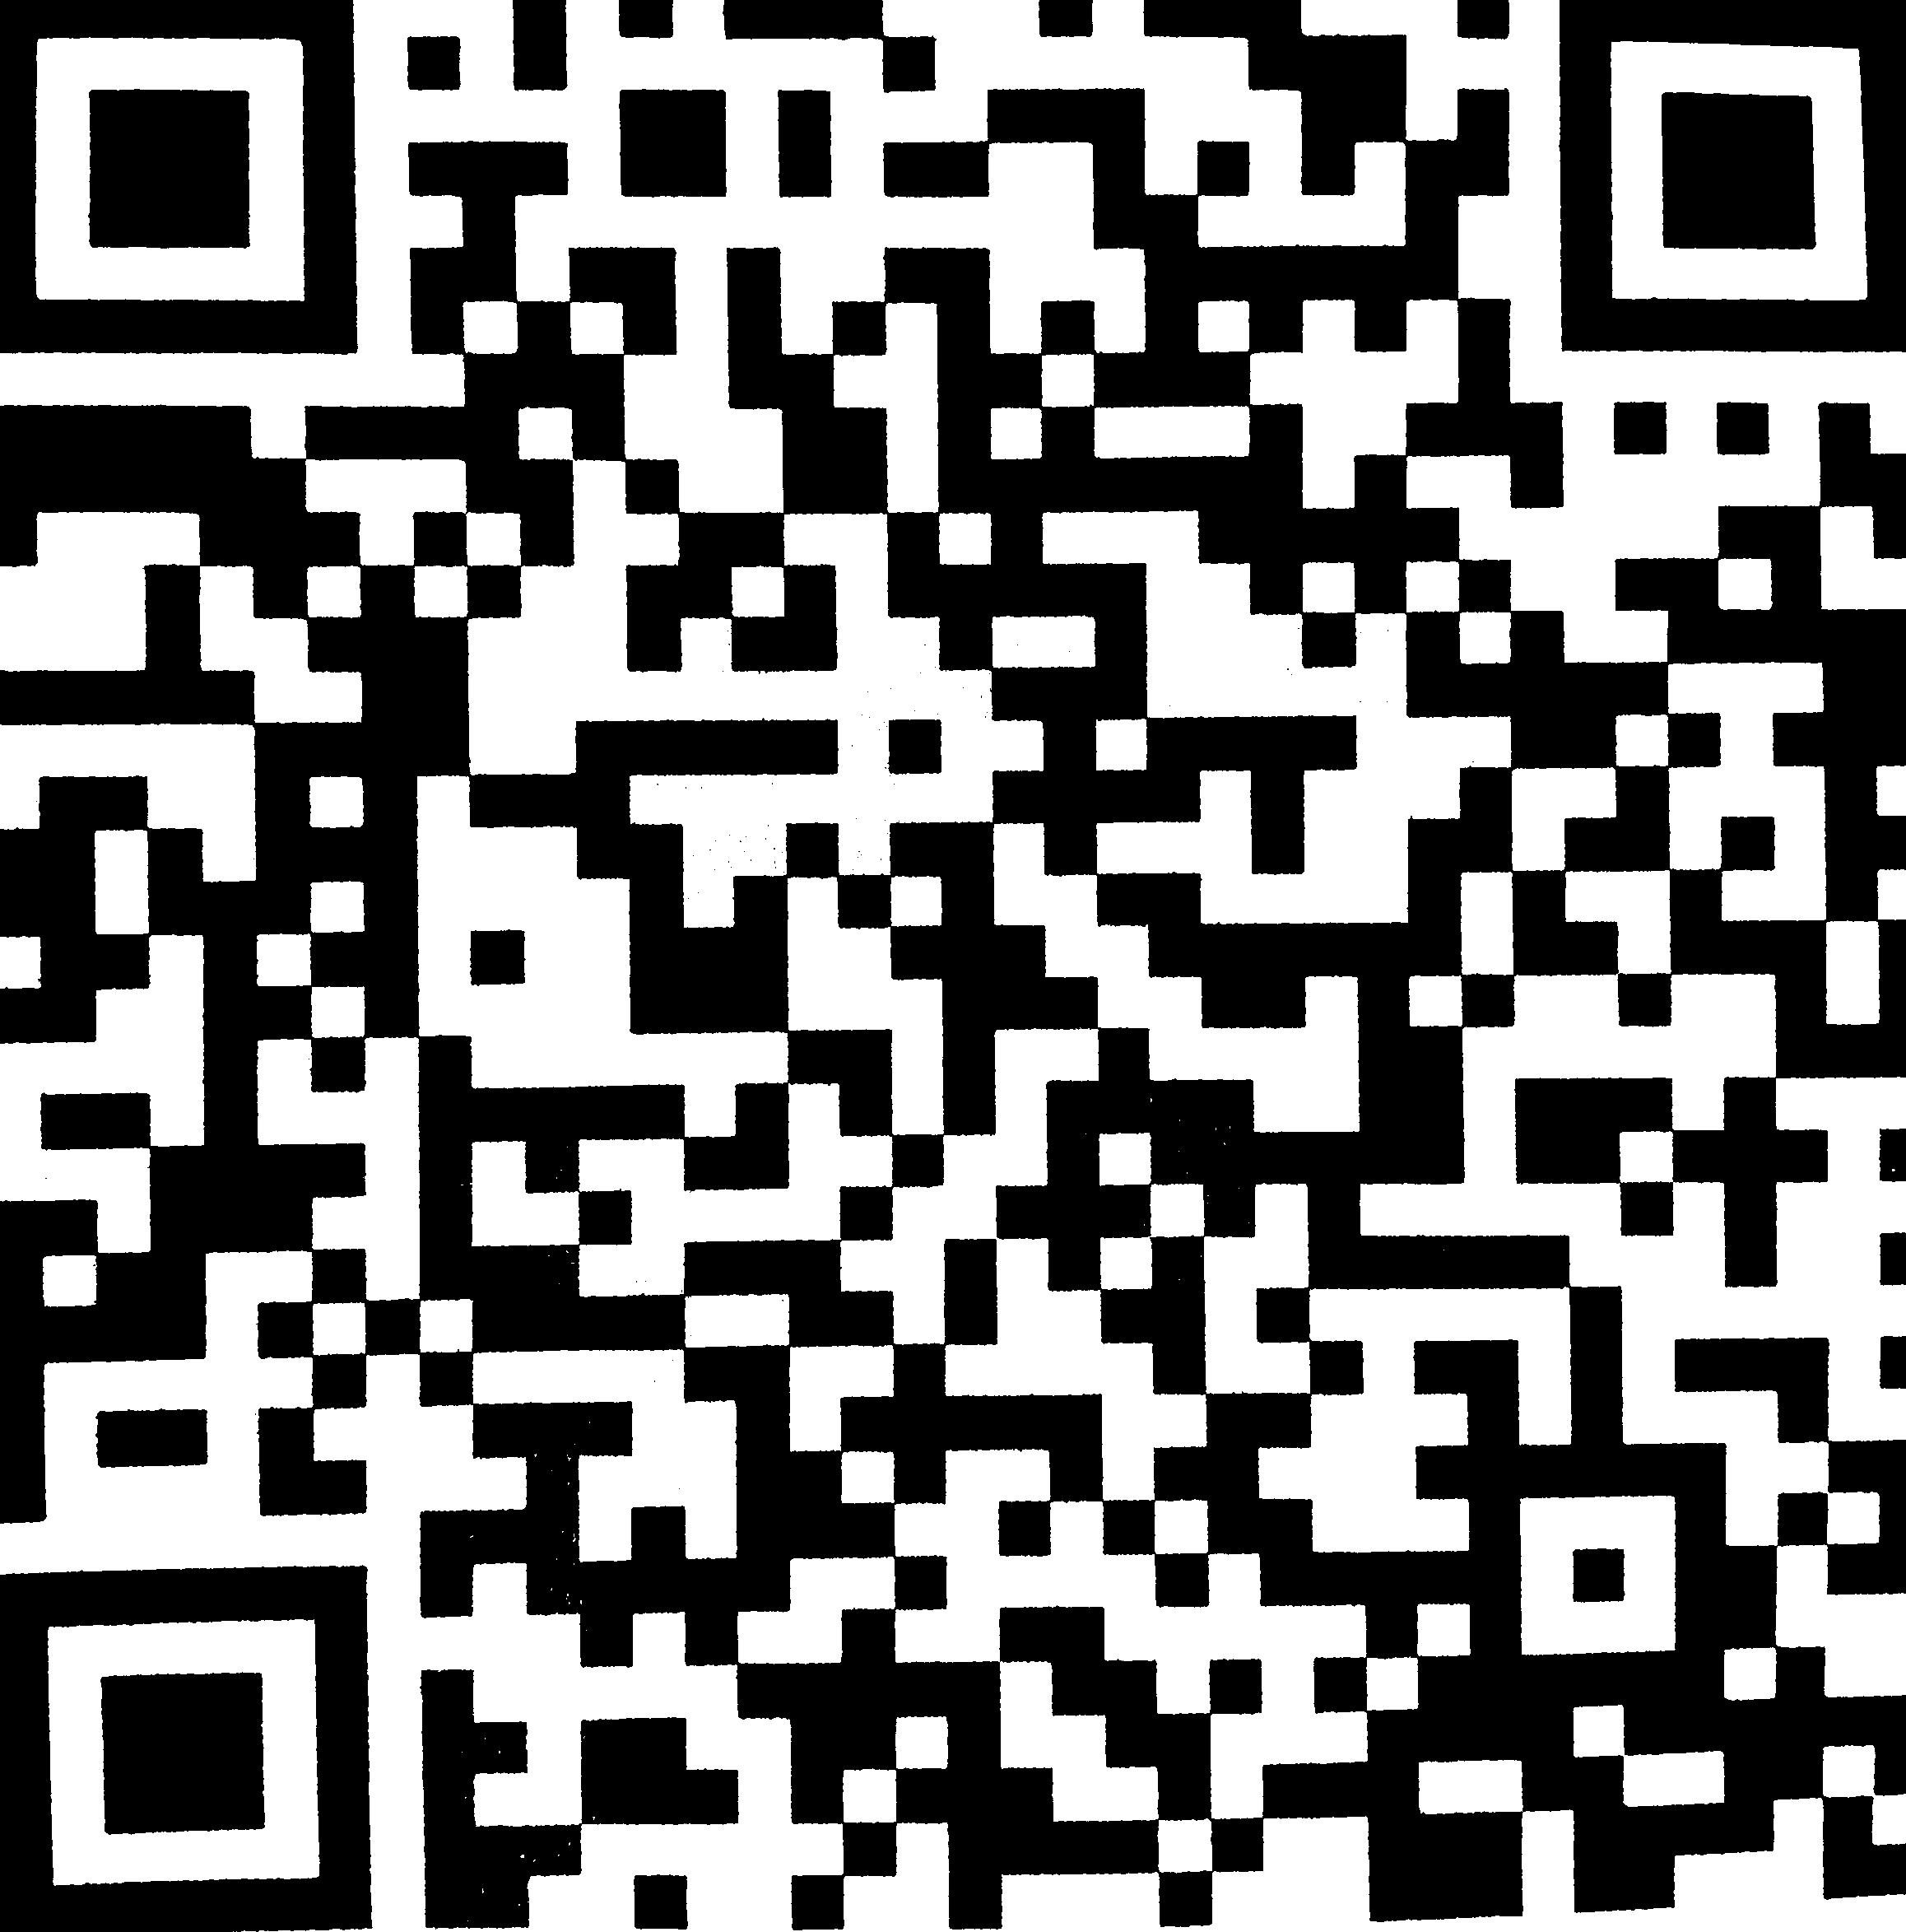
\includegraphics[width=3.68cm]{imagem16-S}}\hfill
\subfloat[]{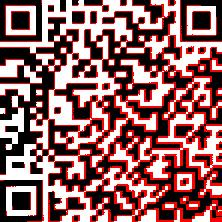
\includegraphics[width=3.68cm]{imagem16-S-diff}}\\
\subfloat[]{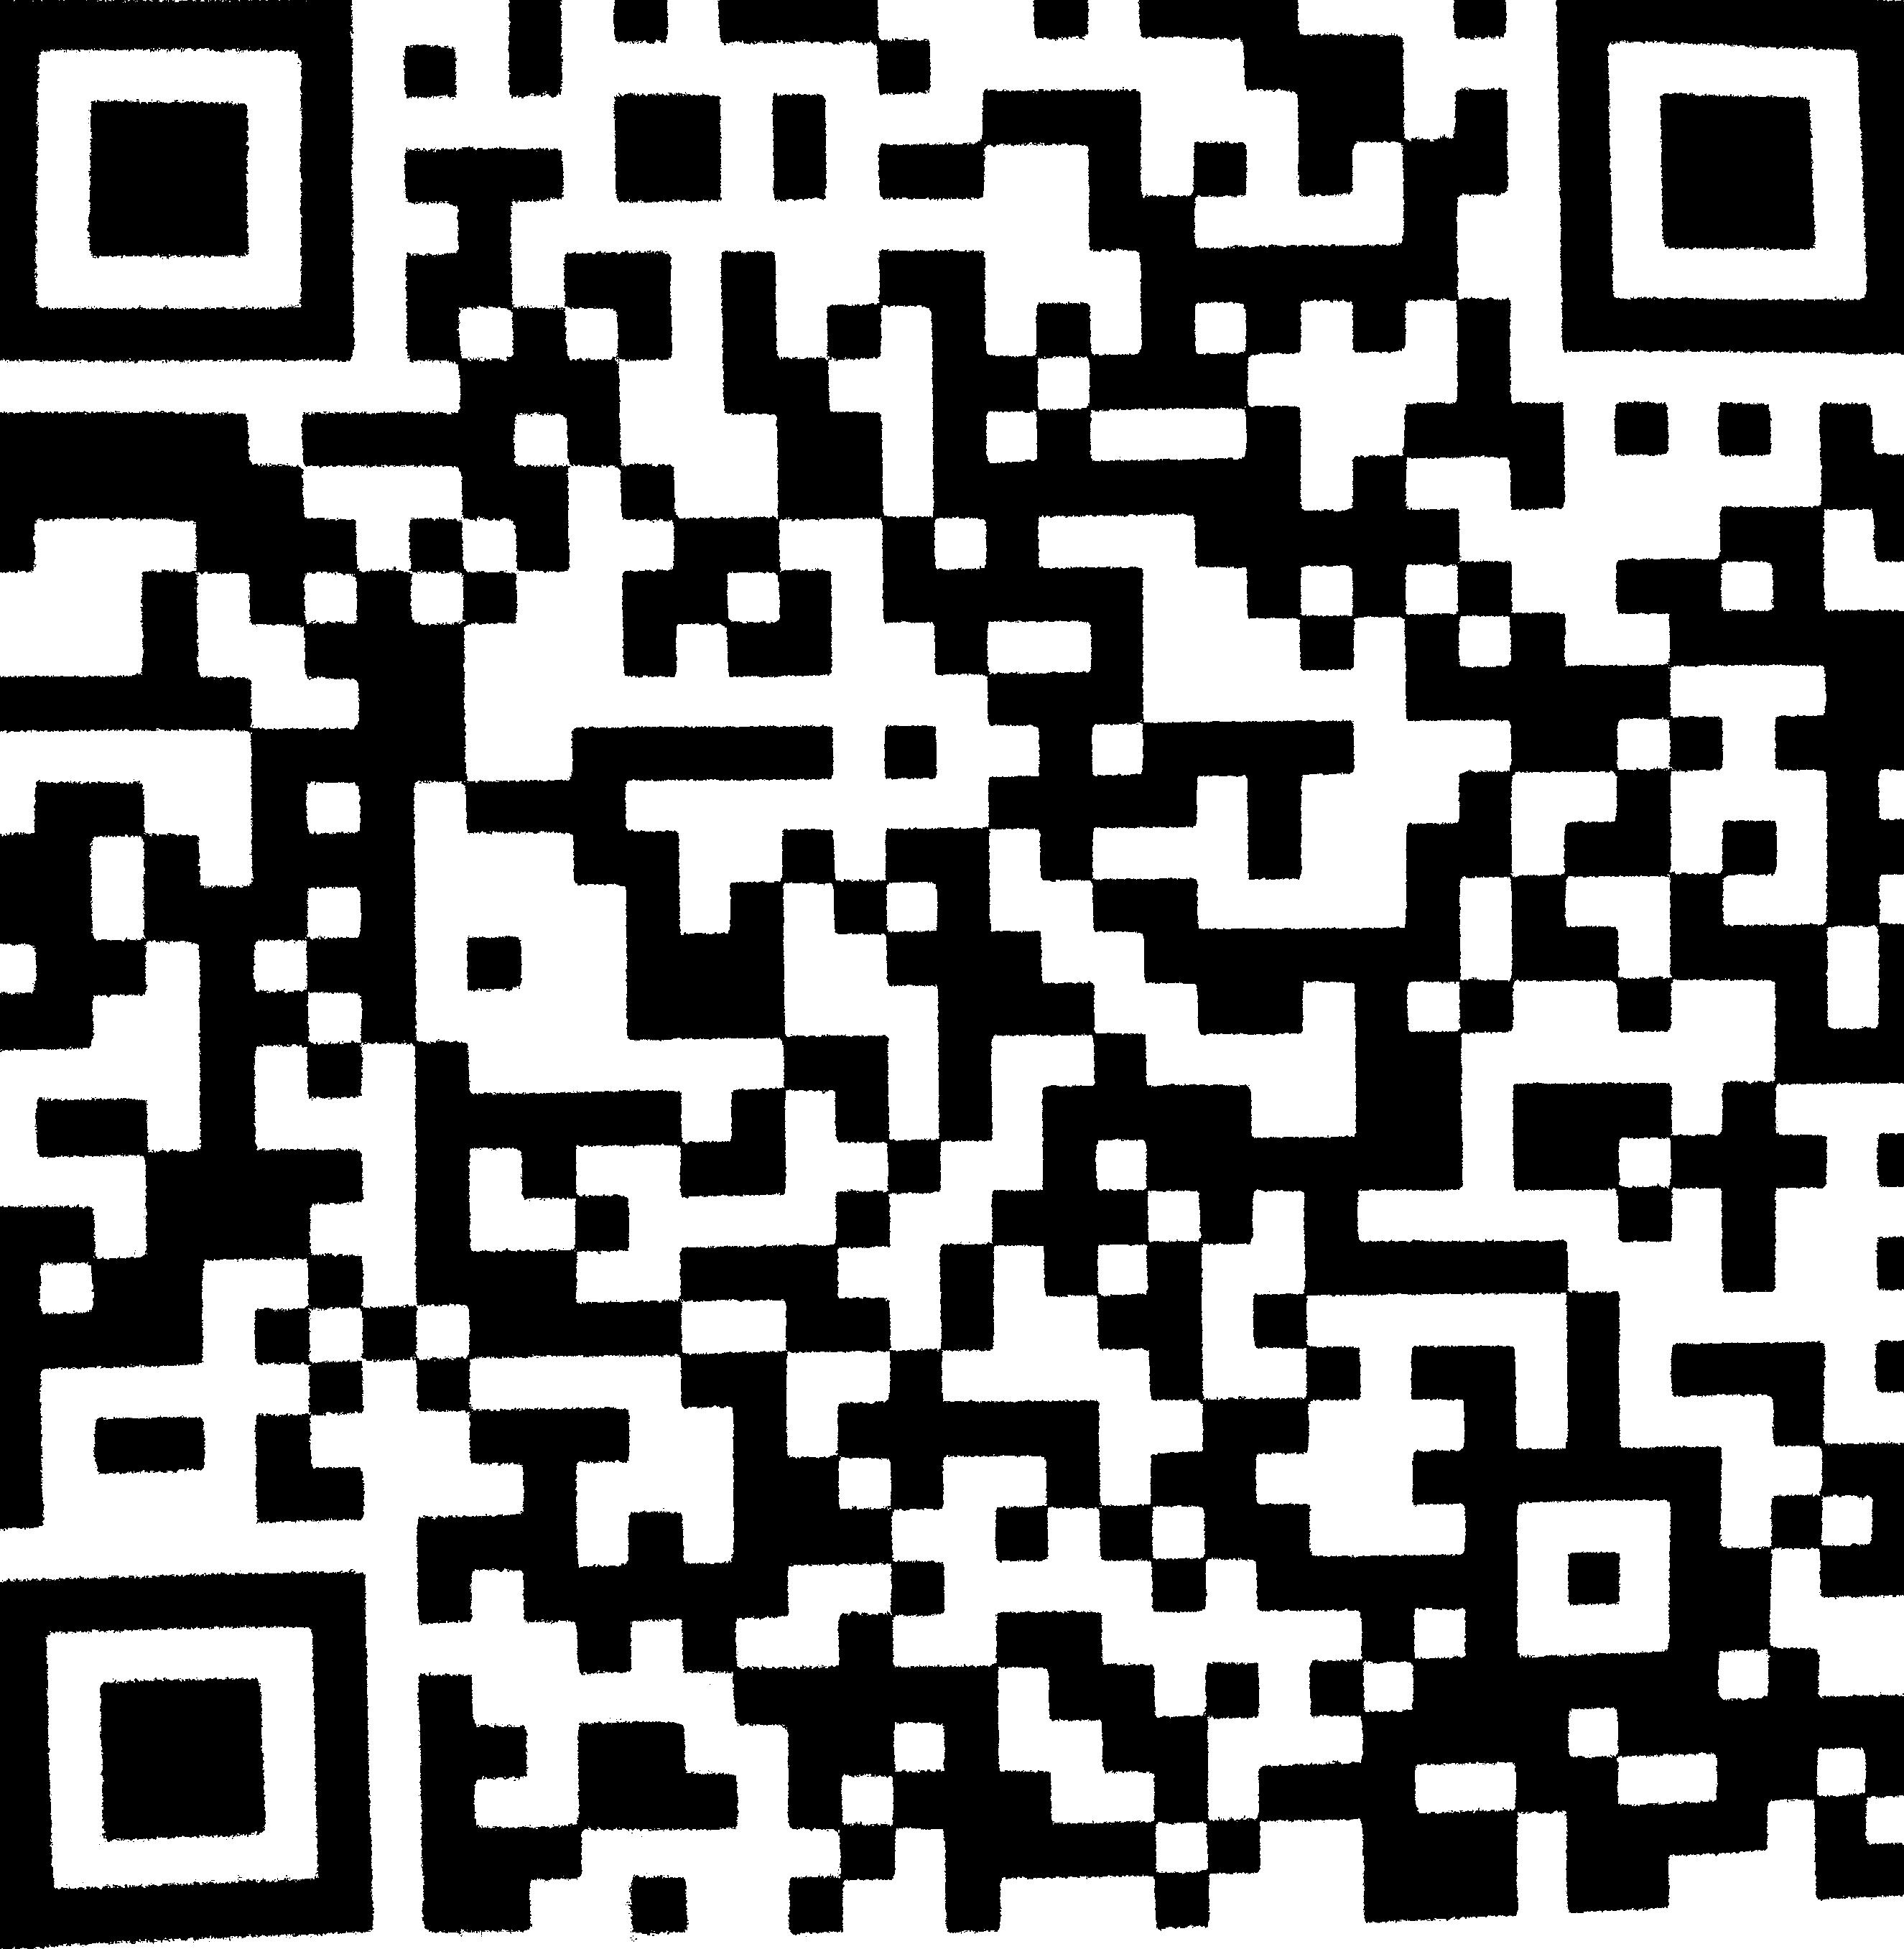
\includegraphics[width=3.68cm]{imagem29-S}}\hfill
\subfloat[]{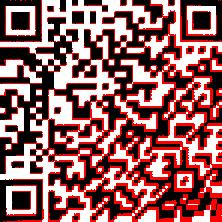
\includegraphics[width=3.68cm]{imagem29-S-diff}}
\vspace{-0.1cm}
\caption{Imagens resultantes da Binarização em Sub-regiões para o QR Code 3 nos padrões de (a) Iluminação 1, (c) Iluminação 2 e (e) Iluminação 3, com suas respectivas imagens diferença em (b), (d) e (f).} \label{figS}
\end{minipage}

\vspace{0.4cm}
dos para os padrões Iluminação 1 e 2, haja vista que as intensidades dos píxeis encontram-se melhor distribuídas ao longo da escala de cinza, como se verifica nos histogramas da Figura \ref{exemplo}. Esse comportamento não ocorre para o padrão de Iluminação 3, pois, devido à sua natureza escura, técnicas que envolvem somente uma etapa, como como \emph{LF} e \emph{LV}, são insatisfatórias, já que é necessário primeiro otimização do contraste da imagem, seja por meio da equalização de histograma ou pela análise em subregiões, das quais, individualmente, espera-se melhor distribuição das intensidades dos píxeis.


\vspace{0.4cm}
\hspace{-0.38cm}
\begin{minipage}[h]{\columnwidth}
\begin{scriptsize} 
\def\arraystretch{1.38}
\captionsetup{type=table}
\caption{Erro percentual de cada método aplicado e método eficaz para as imagens de QR Code submetidas ao padrão de Iluminação 1.} \label{tabP1} \vspace{-0.2cm}
\resizebox{\textwidth}{!}{ %
\begin{tabular}{c c c c c c} \toprule
\textbf{Nome do QR Code}&\textbf{LF(\%)}&\textbf{LV(\%)}&\textbf{EH(\%)}&\textbf{S(\%)}&\textbf{Método Eficaz} \\\midrule
QR Code 1 & 5,45\% & 5,57\% & 7,95\% & 5,60\% & LF \\
QR Code 2 & 11,17\% & 11,14\% & 11,34\% & 11,15\% & LV \\
QR Code 3 & 15,27\% & 13,97\% & 14,26\% & 13,66\% & S \\
QR Code 4 & 38,67\% & 14,20\% & 15,71\% & 14,22\% & LV \\
QR Code 5 & 11,77\% & 12,92\% & 12,16\% & 12,13\% & LF \\
QR Code 6 & 21,00\% & 21,15\% & 21,03\% & 21,11\% & LF \\
QR Code 7 & 31,53\% & 30,97\% & 31,36\% & 31,57\% & LV \\
QR Code 8 & 40,00\% & 35,81\% & 35,79\% & 36,53\% & EH \\
QR Code 9 & 8,83\% & 7,65\% & 9,83\% & 7,64\% & S \\
QR Code 10 & 27,59\% & 25,63\% & 26,40\% & 27,99\% & LV \\
QR Code 11 & 47,86\% & 47,59\% & 47,28\% & 47,77\% & EH \\
QR Code 12 & 47,62\% & 45,32\% & 45,22\% & 45,29\% & EH \\
QR Code 13 & 34,76\% & 28,69\% & 28,83\% & 29,29\% & LV \\\bottomrule
\end{tabular}%
}
\end{scriptsize}
\end{minipage}

\vspace{0.5cm}
\hspace{-0.38cm}
\begin{minipage}[h]{\columnwidth}
\begin{scriptsize} 
\def\arraystretch{1.35}
\captionsetup{type=table}
\caption{Erro percentual de cada método aplicado e método eficaz para as imagens de QR Code submetidas ao padrão de Iluminação 2.} \label{tabP2} \vspace{-0.2cm}
\resizebox{\textwidth}{!}{ %
\begin{tabular}{c c c c c c} \toprule
\textbf{Nome do QR Code}&\textbf{LF(\%)}&\textbf{LV(\%)}&\textbf{EH(\%)}&\textbf{S(\%)}&\textbf{Método Eficaz} \\\midrule
QR Code 1 & 10,97\% & 10,97\% & 10,78\% & 10,98\% & EH \\
QR Code 2 & 7,43\% & 7,86\% & 7,60\% & 7,99\% & LF \\
QR Code 3 & 20,33\% & 20,73\% & 20,33\% & 21,00\% & LF \\
QR Code 4 & 21,02\% & 20,75\% & 19,91\% & 21,24\% & EH \\
QR Code 5 & 44,49\% & 38,11\% & 37,88\% & 38,73\% & EH \\
QR Code 6 & 22,23\% & 24,32\% & 24,10\% & 25,28\% & LF \\
QR Code 7 & 25,61\% & 25,97\% & 25,68\% & 26,26\% & LF \\
QR Code 8 & 34,25\% & 26,02\% & 26,04\% & 24,43\% & S \\
QR Code 9 & 37,59\% & 38,72\% & 38,72\% & 38,98\% & LF \\
QR Code 10 & 22,32\% & 22,45\% & 22,51\% & 21,76\% & S \\
QR Code 11 & 45,92\% & 45,91\% & 45,88\% & 45,61\% & S \\
QR Code 12 & 35,88\% & 35,85\% & 36,55\% & 35,39\% & S \\
QR Code 13 & 47,12\% & 51,13\% & 49,16\% & 49,05\% & LF \\\bottomrule
\end{tabular}%
}
\end{scriptsize}
\end{minipage}

\vspace{0.5cm}
\hspace{-0.38cm}
\begin{minipage}[h]{\columnwidth}
\begin{scriptsize} 
\def\arraystretch{1.35}
\captionsetup{type=table}
\caption{Erro percentual de cada método aplicado e método eficaz para as imagens de QR Code submetidas ao padrão de Iluminação 3.} \label{tabP3} \vspace{-0.2cm}
\resizebox{\textwidth}{!}{ %
\begin{tabular}{c c c c c c} \toprule
\textbf{Nome do QR Code}&\textbf{LF(\%)}&\textbf{LV(\%)}&\textbf{EH(\%)}&\textbf{S(\%)}&\textbf{Método Eficaz} \\\midrule
QR Code 1 & 50,18\% & 12,95\% & 19,76\% & 10,08\% & S \\
QR Code 2 & 50,14\% & 17,52\% & 19,01\% & 16,21\% & S \\
QR Code 3 & 49,89\% & 34,73\% & 34,24\% & 23,43\% & S \\
QR Code 4 & 50,92\% & 22,52\% & 22,43\% & 11,45\% & S \\
QR Code 5 & 49,10\% & 37,85\% & 37,80\% & 22,38\% & S \\
QR Code 6 & 49,44\% & 31,20\% & 31,58\% & 20,69\% & S \\
QR Code 7 & 48,97\% & 34,08\% & 34,11\% & 31,68\% & S \\
QR Code 8 & 48,47\% & 19,39\% & 11,75\% & 12,04\% & EH \\
QR Code 9 & 49,76\% & 26,38\% & 21,33\% & 27,20\% & EH \\
QR Code 10 & 48,68\% & 25,77\% & 25,27\% & 23,97\% & S \\
QR Code 11 & 50,53\% & 46,09\% & 46,09\% & 41,15\% & S \\
QR Code 12 & 49,33\% & 38,25\% & 45,57\% & 47,12\% & LV \\
QR Code 13 & 49,12\% & 45,98\% & 44,43\% & 28,88\% & S \\\bottomrule
\end{tabular}%
}
\end{scriptsize}
\end{minipage}


\section{CONCLUSÕES}
A tecnologia de reconhecimento de QR Code enfrenta problemas significativos provocados principalmente pelo ambiente de filmagem, a exemplo disso cita-se a iluminação irregular no momento da captura da imagem. Por isso, é necessária a aplicação de um método de binarização, nesse sentido, no artigo foram desenvolvidos e propostos três alternativas para esse processamento. Submetendo-se capturas de símbolos QR em três distintos padrões de luminosidade aos métodos desenvolvidos, observou-se a melhor eficácia de métodos que levavam em consideração características mais gerais sobre padrões mais claros, como os \emph{Métodos LF} e \textit{LV}, enquanto que para iluminações de irregularidade extrema ou escuras, métodos preconizando etapas otimização de contraste (\emph{Métodos EH}) ou de binarização localizada (\emph{Métodos S}) trouxeram melhores resultados, pois proporcionaram, à binarização, um limiar mais adequado. Assim, ainda que apresentando certa porcentagem de erro, o método eficaz permite a identificação do símbolo QR.

%==================================
% REFERÊNCIAS
%==================================
\begin{thebibliography}{9} % apague as linhas abaixo e insira aqui bibliografia

\bibitem{denso}	
    DENSO WAVE Incorporated,
    “Basic Info”. 
    Disponível em \url{http://www.denso-wave.com/en/adcd/fundamental/index.html}. Acesso em jun. 2019.

\bibitem{jin-wei}
J. W. Wei, S. G. Dai, P. A. Mu, 
"QR code correction and positioning method based on morphology and Hough transform", 
\emph{Computer and Information
Technology}, Shanghai, China, 2010.

\bibitem{k-suran}
K. Suran, 
"QR Code Image Correction based on Corner Detection and Convex Hull Algorithm". 
\emph{Journal of Multimedia}, Zhejiang, China, 2013.

\bibitem{w-chen}
 W. B. Chen, G. B. Yang, L. Feng, 
"A low complexity image preprocessing method for QR code recognition", 
\emph{Journal of Hunan University}, Hunan, China, 2012.

\bibitem{j-chen}
C. Jin, J. H. Yuan, L. L. Li, E. Y. Chen, G. Han, T. Tang, 
"One of the image correction algorithms of QR code and its implementation
based on wavelet transform".
\emph{2012 IEEE 3rd International Conference on
Software Engineering and Service Science}, Chongqing, China, 2012.

\bibitem{qr-tutorial}
	"QR Code Tutorial", 2015.
	Disponível em \url{https://www.thonky.com/qr-code-tutorial/}. Acesso em jul. 2019.

\bibitem{chines}
  M. Li, P. Cao, L. Feng, L. Yu, J. Chen, J. Wang,
   “The research of QR code image correction based on image gray feature”,
   \emph{ 2017 First International Conference on Electronics Instrumentation \& Information Systems (EIIS)}, Harbin, China, June 2017.

\bibitem{octave}
"Octave Forge". 
Disponível em \url{https://octave.sourceforge.io/}. Acesso em jul. 2019.

\bibitem{gonzales}	
    R. C. Gonzales, R. E. Woods,
    “Processamento Digital de Imagens”, 
    3. ed. , São Paulo, Pearson Prentice Hall, 2010.

\end{thebibliography}

%--- FIM ---

\end{multicols}
\end{document}
